\chapter{Beyond Hermitian: Complex Potentials and PT Symmetry}\label{ch:non-hermitian}

\begin{chapterintro}
Every Hamiltonian you have met so far had a real potential $V(x)$. That was no accident. A real potential makes the Hamiltonian Hermitian, and Hermitian operators have real eigenvalues and orthogonal eigenvectors (Chapter~\ref{ch:eigen}). Physically, a real potential conserves probability: a particle in a box stays in the box forever. Some physical systems do not conserve probability. A neutron passing through a nucleus can be absorbed. Light travelling down an optical fiber with a lossy coating fades. A laser medium amplifies. Physicists describe such systems by letting the potential have an \emph{imaginary} part. In this chapter you will learn what happens to energy levels when you do that: they become complex numbers, their imaginary parts describe decay or growth, and the familiar rules of perturbation theory acquire a crucial minus sign.

That minus sign has consequences. Under an imaginary perturbation, energy levels \emph{attract} instead of repelling; the real shifts of all levels add up to exactly zero; a perturbation of a special symmetry (called PT symmetry) keeps the spectrum real until two levels collide; and beyond that collision the spectrum turns complex and perturbation theory fails completely. We will derive each of these facts line by line and check them on examples small enough to do by hand.

Where this shows up in the paper: Sec.~II E of the paper defines two non-Hermitian model classes, a ``PT-odd'' class and an ``absorptive-even'' class, whose real level shifts are given by the second-order formula of its Eq.~(5). Sec.~V and Sec.~V A dissect what went wrong when those models were fitted to the zeros: an optimizer harvested numerical noise through an ``exactly-null constant mode'', and second-order perturbation theory was used far outside its range of validity, as Fig.~5 shows. The formulas and safeguards of those sections are explained here; the fitting machinery itself is in Chapter~\ref{ch:fitting} and the full reading of Sec.~V in Chapter~\ref{ch:paper-spurious-floor}.
\end{chapterintro}

\begin{prerequisites}
\item Chapter~\ref{ch:complex}: complex numbers, real and imaginary parts, complex conjugate $\bar z$ or $z^*$, modulus $|z|$, $e^{i\theta}$, and $|e^{i\theta}|=1$.
\item Chapter~\ref{ch:series}: Taylor series and radius of convergence.
\item Chapter~\ref{ch:asymptotics}: big-O notation, floating-point numbers, machine epsilon ($2.2\times10^{-16}$ in double precision, $1.2\times10^{-7}$ in single precision, float32).
\item Chapter~\ref{ch:linear-algebra}: matrices, transpose, conjugate transpose, inner products, norms.
\item Chapter~\ref{ch:eigen}: eigenvalues and eigenvectors, the characteristic polynomial for $2\times2$ and $3\times3$ matrices, Hermitian matrices have real eigenvalues, numerical eigensolvers, matching eigenvectors by overlap.
\item Chapter~\ref{ch:schrodinger}: the time-dependent and time-independent Schr\"odinger equations in units $\hbar=2m=1$, normalization, Hermitian operators.
\item Chapter~\ref{ch:bound-states}: the infinite square well on $[-L,L]$, parity of states in an even potential, the harmonic oscillator.
\item Chapter~\ref{ch:perturbation}: first- and second-order perturbation theory for a real (Hermitian) perturbation, matrix elements, the condition for validity.
\item First-year physics: exponential decay, half-life.
\end{prerequisites}

%======================================================================
\section{Complex potentials and decay}\label{sec:non-hermitian-decay}
% DYK-BEGIN
\begin{didyouknow}{Escaping Through a Wall}
In 1928 George Gamow, and independently Ronald Gurney and Edward Condon, explained alpha decay as quantum tunneling through the nuclear barrier. Gamow described the decaying state with a complex energy whose imaginary part sets the decay rate. Tunneling explains why alpha-emitter half-lives range from under a microsecond to billions of years, since small changes in energy change the escape probability enormously.
\end{didyouknow}
% DYK-END
%======================================================================

\subsection{Why a potential might be complex}

Recall from Chapter~\ref{ch:schrodinger} the time-dependent Schr\"odinger equation. In the units used throughout this book and in the paper, $\hbar=1$ and $2m=1$, it reads
\begin{equation}
i\,\frac{\partial\Psi}{\partial t} \;=\; -\frac{\partial^2\Psi}{\partial x^2} + V(x)\,\Psi .
\label{eq:non-hermitian-tdse}
\end{equation}
Here $\Psi(x,t)$ is the wavefunction, $x$ is position and $t$ is time. (In this chapter $t$ is a time; in the rest of the book $t$ usually denotes the height of a zeta zero. The context always makes clear which is meant.) By the Born rule, $|\Psi(x,t)|^2$ is the probability density for finding the particle at $x$, so the total probability of finding the particle anywhere is
\begin{equation}
P_{\rm tot}(t) \;=\; \int_{-L}^{L} |\Psi(x,t)|^2\,\dd x ,
\label{eq:non-hermitian-ptot}
\end{equation}
for a particle confined to the box $[-L,L]$ by walls at which $\Psi(\pm L,t)=0$ (Dirichlet walls, Chapter~\ref{ch:bound-states}).

In Chapter~\ref{ch:schrodinger} you saw that $P_{\rm tot}$ stays equal to 1 forever when $V$ is real. Now let us allow the potential to have a real part $V_R(x)$ and an imaginary part $V_I(x)$, both real-valued functions:
\begin{equation}
V(x) = V_R(x) + i\,V_I(x).
\label{eq:non-hermitian-complexV}
\end{equation}
We want to know how $P_{\rm tot}$ changes in time.

\subsection{The rate of change of the total probability}

Differentiate \eqref{eq:non-hermitian-ptot} with respect to $t$. The limits do not depend on $t$, so the derivative goes inside the integral. Since $|\Psi|^2 = \Psi^*\Psi$, the product rule gives
\begin{equation}
\frac{\dd P_{\rm tot}}{\dd t} = \int_{-L}^{L}\left(\Psi^*\frac{\partial\Psi}{\partial t} + \Psi\frac{\partial\Psi^*}{\partial t}\right)\dd x .
\label{eq:non-hermitian-dPdt1}
\end{equation}
From \eqref{eq:non-hermitian-tdse}, dividing by $i$ (that is, multiplying by $-i$, since $1/i=-i$),
\begin{equation}
\frac{\partial\Psi}{\partial t} = -i\left(-\Psi'' + V_R\Psi + iV_I\Psi\right),
\end{equation}
where a prime denotes $\partial/\partial x$. Taking the complex conjugate of both sides (conjugation turns $i$ into $-i$ and leaves the real functions $V_R$, $V_I$ alone):
\begin{equation}
\frac{\partial\Psi^*}{\partial t} = +i\left(-\Psi^{*\prime\prime} + V_R\Psi^* - iV_I\Psi^*\right).
\end{equation}
Now multiply the first by $\Psi^*$ and the second by $\Psi$:
\begin{align}
\Psi^*\frac{\partial\Psi}{\partial t} &= i\Psi^*\Psi'' - iV_R|\Psi|^2 + V_I|\Psi|^2,
\quad\text{(using $-i\cdot i = 1$)}\\
\Psi\frac{\partial\Psi^*}{\partial t} &= -i\Psi\Psi^{*\prime\prime} + iV_R|\Psi|^2 + V_I|\Psi|^2.
\quad\text{(using $i\cdot(-i) = 1$)}
\end{align}
Add them. The $V_R$ terms cancel, and the $V_I$ terms double:
\begin{equation}
\Psi^*\frac{\partial\Psi}{\partial t} + \Psi\frac{\partial\Psi^*}{\partial t}
= i\left(\Psi^*\Psi'' - \Psi\Psi^{*\prime\prime}\right) + 2V_I|\Psi|^2 .
\end{equation}
The bracket is a total derivative. By the product rule,
\begin{equation}
\frac{\partial}{\partial x}\left(\Psi^*\Psi' - \Psi\Psi^{*\prime}\right)
= \Psi^{*\prime}\Psi' + \Psi^*\Psi'' - \Psi'\Psi^{*\prime} - \Psi\Psi^{*\prime\prime}
= \Psi^*\Psi'' - \Psi\Psi^{*\prime\prime}.
\end{equation}
So its integral over $[-L,L]$ is $\bigl[\Psi^*\Psi' - \Psi\Psi^{*\prime}\bigr]_{-L}^{L}$, which is zero because $\Psi$ and $\Psi^*$ vanish at both walls. Substituting into \eqref{eq:non-hermitian-dPdt1}:
\begin{equation}
\boxed{\;\frac{\dd P_{\rm tot}}{\dd t} = 2\int_{-L}^{L} V_I(x)\,|\Psi(x,t)|^2\,\dd x.\;}
\label{eq:non-hermitian-dPdt}
\end{equation}
This is the key result. The real part of the potential never changes the total probability. The imaginary part does: where $V_I<0$ probability drains away (absorption, or loss), and where $V_I>0$ it is created (gain). If $V_I=0$ everywhere we recover conservation of probability.

The commonest special case is a constant negative imaginary part, conventionally written
\begin{equation}
V_I(x) = -\frac{\Gamma}{2}, \qquad \Gamma \text{ a real constant}.
\label{eq:non-hermitian-gamma}
\end{equation}
Then \eqref{eq:non-hermitian-dPdt} becomes $\dd P_{\rm tot}/\dd t = -\Gamma P_{\rm tot}$, whose solution (first-year physics: exponential decay) is
\begin{equation}
P_{\rm tot}(t) = P_{\rm tot}(0)\,e^{-\Gamma t}.
\label{eq:non-hermitian-expdecay}
\end{equation}
For $\Gamma>0$ the particle disappears at rate $\Gamma$; its mean lifetime is $\tau=1/\Gamma$ and its half-life is $t_{1/2}=\log 2/\Gamma$ (natural log, as always in this book). The quantity $\Gamma$ is called the \emph{width}. (The name comes from spectroscopy: a decaying state emits light whose spectral line has a frequency spread proportional to $\Gamma$. We use the word only as a label.) The physical requirement that a lossy medium absorbs rather than amplifies is $\Gamma\ge0$, that is, $V_I\le0$.

\subsection{Stationary states with complex energy}

Recall from Chapter~\ref{ch:schrodinger} that separation of variables, $\Psi(x,t)=\psi(x)e^{-iEt}$, turns \eqref{eq:non-hermitian-tdse} into the time-independent equation $H\psi=E\psi$ with $H=-\dd^2/\dd x^2+V(x)$. Nothing in that step used the reality of $V$, so it still works; but now nothing forces $E$ to be real. Write
\begin{equation}
E = E_R - i\,\frac{\Gamma}{2},
\label{eq:non-hermitian-complexE}
\end{equation}
with $E_R$ and $\Gamma$ real. Then
\begin{equation}
e^{-iEt} = e^{-iE_R t}\,e^{-i(-i\Gamma/2)t} = e^{-iE_Rt}\,e^{-\Gamma t/2},
\end{equation}
because $-i\cdot(-i)=i^2=-1$. Since $|e^{-iE_Rt}|=1$ (Chapter~\ref{ch:complex}),
\begin{equation}
|\Psi(x,t)|^2 = |\psi(x)|^2\,e^{-\Gamma t}.
\end{equation}
So a stationary state with complex energy oscillates at angular frequency $E_R$ (its ``energy level'' in the usual sense) while its probability decays at rate $\Gamma = -2\,\Im E$. The real part of a complex eigenvalue is the level; minus twice the imaginary part is the width.

\subsection{An exact formula for the imaginary part}

There is a neat exact statement. Suppose $H\psi = E\psi$ with $\psi(\pm L)=0$. Multiply by $\psi^*$ and integrate:
\begin{equation}
\int_{-L}^{L}\psi^*\left(-\psi''\right)\dd x + \int_{-L}^{L} V_R|\psi|^2\dd x + i\int_{-L}^{L}V_I|\psi|^2\dd x = E\int_{-L}^{L}|\psi|^2\dd x .
\end{equation}
Integrate the first term by parts: $\int\psi^*(-\psi'')\dd x = -\bigl[\psi^*\psi'\bigr]_{-L}^{L} + \int \psi^{*\prime}\psi'\dd x = \int|\psi'|^2\dd x$, since the boundary term vanishes at the walls. This is real. The second term is real. Only the third is imaginary. Taking the imaginary part of both sides and dividing by $\int|\psi|^2\dd x$:
\begin{equation}
\Im E = \frac{\int_{-L}^{L} V_I(x)|\psi(x)|^2\,\dd x}{\int_{-L}^{L}|\psi(x)|^2\,\dd x}.
\label{eq:non-hermitian-ImE}
\end{equation}
The imaginary part of every eigenvalue is a weighted average of $V_I$, weighted by the probability density of that eigenstate. Two immediate consequences:
\begin{itemize}
\item If $V_I(x)\le0$ everywhere, then $\Im E\le0$ for \emph{every} eigenvalue, so every width is nonnegative. A purely absorbing potential cannot produce a growing state.
\item If $V_I$ is a constant $-\Gamma/2$, then $\Im E=-\Gamma/2$ for every level, exactly. In fact in this case $H = H_R - i\Gamma/2$ where $H_R$ is the real Hamiltonian, so every eigenfunction of $H_R$ with level $E_n$ is an eigenfunction of $H$ with eigenvalue $E_n - i\Gamma/2$. A constant imaginary potential moves every eigenvalue straight down in the complex plane by the same amount and changes nothing else.
\end{itemize}

\subsection{Hermitian or not?}

Recall from Chapter~\ref{ch:schrodinger} that an operator $H$ is Hermitian if $\int f^*(Hg)\,\dd x = \int (Hf)^*g\,\dd x$ for all allowed $f,g$. The kinetic part $-\dd^2/\dd x^2$ passes this test (two integrations by parts), and so does multiplication by a real function. Multiplication by $iV_I$ fails: $\int f^*(iV_Ig)\dd x = i\int f^*V_I g\,\dd x$, while $\int(iV_If)^*g\,\dd x = -i\int f^*V_Ig\,\dd x$. These differ by a sign unless $\int f^*V_Ig\,\dd x=0$. So a Hamiltonian with $V_I\ne0$ is \emph{non-Hermitian}, and the guarantee of real eigenvalues proved in Chapter~\ref{ch:eigen} no longer applies. Equation~\eqref{eq:non-hermitian-ImE} shows exactly how far from real the eigenvalues can be.

\begin{sample}{A leaky level in the running box}
A particle is in the tenth level of the infinite well on $[-L,L]$ with $L=44.883$ (running example RE3). A uniform absorber $V_I=-\Gamma/2$ with $\Gamma=0.02$ is switched on. Find the complex energy, the fraction of probability left at $t=50$, and the half-life.

\textbf{Step 1: the real level.} From Chapter~\ref{ch:bound-states}, the levels of the box are $E_k=(k\pi/2L)^2$. For $k=10$: $E_{10}=(10\pi/89.766)^2 = (0.34998)^2 \approx 0.1225$.

\textbf{Step 2: the complex energy.} A constant imaginary part shifts every eigenvalue by exactly $-i\Gamma/2=-0.01i$, so $E = 0.1225 - 0.01i$.

\textbf{Step 3: survival.} By \eqref{eq:non-hermitian-expdecay}, $P_{\rm tot}(50)/P_{\rm tot}(0)=e^{-0.02\times50}=e^{-1}=0.3679$.

\textbf{Step 4: half-life.} $t_{1/2}=\log2/\Gamma = 0.6931/0.02 = 34.66$.

\[
\boxed{E\approx 0.1225-0.01i,\quad P_{\rm tot}(50)=0.368\,P_{\rm tot}(0),\quad t_{1/2}=34.66}
\]
The width does not depend on which level the particle occupies, because the absorber is uniform.
\end{sample}

\begin{checkpoint}
A potential has $V_I>0$ (gain) in the left half of the box and $V_I<0$ (loss) in the right half. Must the total probability decrease?
\end{checkpoint}
\checkanswer{No. By \eqref{eq:non-hermitian-dPdt} the rate is $2\int V_I|\Psi|^2\,\dd x$; it is positive if the particle is mostly on the left and negative if it is mostly on the right. The sign depends on where the probability sits.}

\begin{keyideas}
\item The real part of a potential conserves probability; the imaginary part changes it at the rate $2\int V_I|\Psi|^2\,\dd x$, \eqref{eq:non-hermitian-dPdt}.
\item A stationary state with $E=E_R-i\Gamma/2$ oscillates at $E_R$ and decays as $e^{-\Gamma t}$; $\Gamma=-2\Im E$ is the width.
\item $\Im E$ is the probability-weighted average of $V_I$, \eqref{eq:non-hermitian-ImE}; if $V_I\le0$ everywhere, all widths are nonnegative.
\item A constant imaginary potential shifts all eigenvalues by the same imaginary constant and leaves their real parts and eigenfunctions unchanged.
\end{keyideas}

%======================================================================
\section{Non-Hermitian matrices}\label{sec:non-hermitian-matrices}
%======================================================================

\subsection{The Hamiltonian in the unperturbed basis}

The paper works with Hamiltonians of the form
\begin{equation}
H = H_0 + iA, \qquad H_0 = -\frac{\dd^2}{\dd x^2} + V(x),
\label{eq:non-hermitian-HiA}
\end{equation}
where $V$ is real (the Wu--Sprung potential, Chapter~\ref{ch:wu-sprung}, or in our examples the box) and $A(x)$ is a \emph{real} function. ``$A$ is a real multiplication operator'' simply means that $A$ acts on a wavefunction by multiplying it by the real function $A(x)$. Comparing with \eqref{eq:non-hermitian-complexV}, $iA$ is an imaginary potential with $V_I = A$; an absorber has $A=-\Gamma/2\le0$.

\begin{pitfall}
The letter $A$ is overloaded in the paper. In Sec.~II C (and in Chapters~\ref{ch:perturbation} and~\ref{ch:fitting}) $A_{nk}$ is the \emph{sensitivity matrix} $\int|\psi_n|^2\phi_k\,\dd x$. In Sec.~II E, Eq.~(5), and in this chapter, $A$ is the real multiplication operator in $H+iA$, and $A_{nm}=\langle n|A|m\rangle$ are its matrix elements between two unperturbed states. Read the subscripts: $A_{nm}$ with two level indices is a matrix element of the operator; $A_{nk}$ with a basis index $k$ is a sensitivity.
\end{pitfall}

Let $\psi_n$, $n=1,2,\dots$, be the normalized eigenfunctions of $H_0$ with levels $E_n$. Because $V$ is real, the $\psi_n$ can be chosen real (here is the argument: $E$ is real because $H_0$ is Hermitian, Chapter~\ref{ch:schrodinger}; if $H_0\psi=E\psi$, conjugating gives $H_0\psi^*=E\psi^*$, because $H_0$ contains no $i$; hence $\Re\psi=(\psi+\psi^*)/2$ and $\Im\psi=(\psi-\psi^*)/(2i)$ are real solutions with the same $E$; they cannot both be zero, since $\psi\ne0$, and a nonzero one can be used as the eigenfunction). Expand any wavefunction as $\psi=\sum_m v_m\psi_m$. The set of all $\psi_m$ is infinite, so this is an infinite sum. Then $H\psi=E\psi$ becomes, after multiplying by $\psi_n$ and integrating over $[-L,L]$ (the inner product with the real function $\psi_n$), the matrix equation $\sum_m M_{nm}v_m = E v_n$ with
\begin{equation}
M_{nm} = \int\psi_n\,(H_0+iA)\,\psi_m\,\dd x = E_n\delta_{nm} + iA_{nm},
\qquad
A_{nm} = \int_{-L}^{L}\psi_n(x)\,A(x)\,\psi_m(x)\,\dd x .
\label{eq:non-hermitian-Anm}
\end{equation}
Here $\delta_{nm}$ is the Kronecker delta: 1 if $n=m$, 0 otherwise. We used $H_0\psi_m = E_m\psi_m$ and $\int\psi_n\psi_m\,\dd x=\delta_{nm}$ (orthonormality). The exact matrix $M_{nm}$ is infinite. On a computer we keep only the lowest $K$ states, $m=1,\dots,K$. This truncation is an approximation: it is accurate for levels well below $E_K$ when their couplings to the discarded states are small, and we will see in Section~\ref{sec:non-hermitian-sumrule} what it does to the levels near the cutoff. In this truncated basis write $D=\mathrm{diag}(E_1,\dots,E_K)$ and let $\mathsf{A}$ be the $K\times K$ matrix of the $A_{nm}$. Then
\begin{equation}
M = D + i\mathsf{A}.
\label{eq:non-hermitian-M}
\end{equation}

Two properties of $\mathsf A$ follow at once from \eqref{eq:non-hermitian-Anm}. Every factor in the integrand is real, so $A_{nm}$ is \textbf{real}. And swapping $n$ and $m$ swaps two real factors that commute, so $A_{mn}=A_{nm}$: $\mathsf A$ is \textbf{symmetric}. Hence $M^\top = D + i\mathsf A^\top = M$: the matrix is symmetric. But its conjugate transpose is $M^\dagger = D - i\mathsf A \ne M$ (unless $\mathsf A=0$). A \emph{complex symmetric} matrix is not Hermitian, and none of the theorems of Chapter~\ref{ch:eigen} about real eigenvalues apply to it.

\subsection{Eigenvalues of a $2\times2$ non-Hermitian matrix}

Recall from Chapter~\ref{ch:eigen} that the eigenvalues of a matrix $M$ are the roots of $\det(M-\lambda I)=0$. For a general $2\times2$ matrix,
\begin{equation}
\det\begin{pmatrix} M_{11}-\lambda & M_{12}\\ M_{21} & M_{22}-\lambda\end{pmatrix}
= \lambda^2 - (M_{11}+M_{22})\lambda + (M_{11}M_{22}-M_{12}M_{21}) = 0,
\end{equation}
so by the quadratic formula
\begin{equation}
\lambda_\pm = \frac{M_{11}+M_{22}}{2} \pm \frac12\sqrt{(M_{11}-M_{22})^2 + 4M_{12}M_{21}} .
\label{eq:non-hermitian-2x2}
\end{equation}
(To get the discriminant: $(M_{11}+M_{22})^2 - 4(M_{11}M_{22}-M_{12}M_{21}) = (M_{11}-M_{22})^2+4M_{12}M_{21}$.) When the discriminant is a negative real number or a complex number, the eigenvalues are complex; the square root of a complex number is defined as in Chapter~\ref{ch:complex}.

\begin{sample}{Eigenvalues of a complex symmetric matrix}
Find the eigenvalues of $M=\begin{pmatrix}1 & 2i\\ 2i & 3\end{pmatrix}$ and check that they add up to the sum of the diagonal entries.

\textbf{Step 1.} $M_{11}+M_{22}=4$ and $(M_{11}-M_{22})^2 = 4$.

\textbf{Step 2.} $4M_{12}M_{21}=4(2i)(2i)=16i^2=-16$.

\textbf{Step 3.} The discriminant is $4-16=-12$, whose square root is $i\sqrt{12}=2\sqrt3\,i$.

\textbf{Step 4.} $\lambda_\pm = 2 \pm \tfrac12(2\sqrt3\, i) = 2\pm\sqrt3\,i$.

\textbf{Step 5.} $\lambda_++\lambda_-=4=1+3$.
\[
\boxed{\lambda_\pm = 2 \pm 1.7321\,i}
\]
Compare the Hermitian matrix $\begin{pmatrix}1&2\\2&3\end{pmatrix}$: its discriminant is $4+16=20>0$ and its eigenvalues $2\pm\sqrt5$ are real. Multiplying the off-diagonal entries by $i$ changed $+16$ into $-16$. That single sign is the theme of this chapter.
\end{sample}

\subsection{Three general facts about eigenvalues}

\paragraph{Fact 1: the trace is the sum of the eigenvalues.} The \emph{trace} of a square matrix, $\mathrm{tr}\,M=\sum_n M_{nn}$, is the sum of its diagonal entries. For $2\times2$ matrices, adding the two roots in \eqref{eq:non-hermitian-2x2} cancels the square roots and gives $\lambda_++\lambda_-=M_{11}+M_{22}$. The same is true for any size.

\begin{beyond}
\textbf{Taken on trust:} for any $K\times K$ matrix (real or complex, Hermitian or not), the $K$ eigenvalues, counted with multiplicity, satisfy $\lambda_1+\dots+\lambda_K=\mathrm{tr}\,M$. The proof compares the coefficient of $\lambda^{K-1}$ in two expressions for $\det(\lambda I - M)$: the factorization $\prod_i(\lambda-\lambda_i)$ (which needs the fundamental theorem of algebra) gives $-\sum_i\lambda_i$, and the permutation expansion of the determinant gives $-\sum_n M_{nn}$, because only the product of diagonal entries contains $K-1$ factors of $\lambda$. See \cite{strang} or \cite{rhb}. You prove the $3\times3$ case by hand in Problem 27.
\end{beyond}

For $M=D+i\mathsf A$ the trace is $\sum_n E_n + i\sum_n A_{nn}$. Taking real parts:
\begin{equation}
\sum_{\text{all eigenvalues}}\Re\lambda \;=\; \sum_{n=1}^{K}E_n \qquad\text{(exact, for any $\mathsf A$)}.
\label{eq:non-hermitian-tracerule}
\end{equation}
However large the imaginary perturbation, the real parts of the eigenvalues of the truncated matrix always add up to the sum of the unperturbed levels. We will meet this again as the sum rule of Section~\ref{sec:non-hermitian-sumrule}.

\paragraph{Fact 2: conjugating the matrix conjugates the eigenvalues.} Let $\bar M$ be the matrix whose entries are the complex conjugates of those of $M$. If $Mv=\lambda v$, conjugate every component: $\bar M\bar v = \bar\lambda\bar v$. So $\bar\lambda$ is an eigenvalue of $\bar M$. Now apply this to $M(c)=D+ic\mathsf A$ with a real parameter $c$ multiplying the perturbation. Since $D$ and $\mathsf A$ are real,
\begin{equation}
\overline{M(c)} = D - ic\mathsf A = M(-c).
\end{equation}
So the eigenvalues of $M(-c)$ are the conjugates of those of $M(c)$. Conjugation keeps real parts and flips imaginary parts. Therefore:
\begin{equation}
\text{the set of real parts is even in } c,\qquad \text{the set of imaginary parts is odd in } c.
\label{eq:non-hermitian-parity-in-c}
\end{equation}
This is exact, not perturbative. It already tells you that if real shifts can be expanded in powers of $c$, they contain only even powers: $c^2$, $c^4$, and so on. There can be no real shift linear in $c$.

\paragraph{Fact 3: an absorbing $A$ gives nonnegative widths.} The matrix version of \eqref{eq:non-hermitian-ImE} is short. If $Mv=\lambda v$, multiply on the left by the conjugate transpose $v^\dagger$: $v^\dagger D v + i\,v^\dagger\mathsf Av = \lambda\,v^\dagger v$. Both $v^\dagger Dv=\sum E_n|v_n|^2$ and $v^\dagger\mathsf Av$ are real (the latter because $\mathsf A$ is real symmetric, hence Hermitian). Divide both sides by $v^\dagger v=\sum_n|v_n|^2$, which is a positive real number because $v\ne0$:
\[
\lambda = \frac{v^\dagger Dv}{v^\dagger v} + i\,\frac{v^\dagger\mathsf Av}{v^\dagger v}.
\]
The first term is real and the second is $i$ times a real number, so taking the imaginary part of both sides gives $\Im\lambda = v^\dagger\mathsf A v/v^\dagger v$. Moreover $v^\dagger\mathsf Av=\int|\sum_n v_n\psi_n|^2A(x)\,\dd x$ by \eqref{eq:non-hermitian-Anm}, which is $\le0$ if $A(x)\le0$ everywhere. So even in a truncated basis, a pointwise-absorbing $A$ gives $\Im\lambda\le0$ for every eigenvalue.

\begin{checkpoint}
For $M(c)=D+ic\mathsf A$ with real $D$ and $\mathsf A$, a computer reports an eigenvalue $3.0+0.2i$ at $c=0.1$. Name an eigenvalue of $M(-0.1)$ without computing anything.
\end{checkpoint}
\checkanswer{$3.0-0.2i$, the complex conjugate, by Fact 2.}

\begin{keyideas}
\item In the real eigenbasis of $H_0$, the Hamiltonian $H_0+iA$ becomes $M=D+i\mathsf A$ with $\mathsf A$ real and symmetric: $M$ is complex symmetric, not Hermitian.
\item Multiplying off-diagonal couplings by $i$ turns $+4M_{12}M_{21}$ into a negative number in the discriminant, so eigenvalues can become complex.
\item The real parts of all eigenvalues add up to $\sum E_n$ exactly, \eqref{eq:non-hermitian-tracerule}.
\item Real parts are even in the perturbation strength and imaginary parts odd, \eqref{eq:non-hermitian-parity-in-c}.
\end{keyideas}

%======================================================================
\section{Perturbation theory for a non-Hermitian perturbation}\label{sec:non-hermitian-perturb}
%======================================================================

\subsection{Rederiving second order without assuming Hermiticity}

In Chapter~\ref{ch:perturbation} you derived, for a real perturbation $\delta V$ with matrix elements $V_{nm}=\langle n|\delta V|m\rangle$,
\begin{equation}
\delta E_n \approx V_{nn} + \sum_{m\ne n}\frac{|V_{nm}|^2}{E_n-E_m}.
\label{eq:non-hermitian-hermitianPT}
\end{equation}
It is tempting to substitute $\delta V\to iA$ and write $|V_{nm}|^2=|iA_{nm}|^2=|A_{nm}|^2$. That gives the \emph{wrong sign}. The reason is that the derivation of \eqref{eq:non-hermitian-hermitianPT} used Hermiticity at one point, to rewrite a product $V_{nm}V_{mn}$ as $|V_{nm}|^2$. For a non-Hermitian perturbation that step is false. So let us redo the derivation from scratch, for an arbitrary perturbation matrix $W$, in the matrix language of \eqref{eq:non-hermitian-M}.

\textbf{Setup.} Let $M = D + \epsilon W$, where $D=\mathrm{diag}(E_1,\dots,E_K)$ has distinct entries, $W$ is any $K\times K$ matrix (complex, not necessarily Hermitian or symmetric), and $\epsilon$ is a small bookkeeping parameter that we set to 1 at the end. Fix one level $n$. At $\epsilon=0$, the eigenvector belonging to $E_n$ is the unit vector $e_n$ (1 in position $n$, zeros elsewhere). We assume, as in Chapter~\ref{ch:perturbation}, that for small $\epsilon$ there is an eigenvalue $E(\epsilon)$ close to $E_n$ whose eigenvector $v(\epsilon)$ is close to $e_n$, both depending smoothly on $\epsilon$.

\begin{beyond}
\textbf{Taken on trust:} for a \emph{nondegenerate} eigenvalue (one that is a simple root of the characteristic polynomial), the eigenvalue and a suitably normalized eigenvector are smooth (indeed analytic) functions of $\epsilon$ near $\epsilon=0$. This is a theorem of matrix perturbation theory; see \cite{trefethen}. It fails at degeneracies, which is exactly where we will see perturbation theory break down in Section~\ref{sec:non-hermitian-exact}.
\end{beyond}

\textbf{Normalization choice.} Since $v$ is close to $e_n$, its $n$-th component is not zero, and we can scale $v$ so that $v_n=1$ exactly. (Eigenvectors can be multiplied by any nonzero number.)

\textbf{Row $n$ of the eigen-equation.} The $n$-th component of $Mv=Ev$ is $\sum_m M_{nm}v_m = E\,v_n$. With $M_{nm} = E_n\delta_{nm}+\epsilon W_{nm}$ and $v_n=1$:
\begin{equation}
E_n + \epsilon W_{nn} + \epsilon\sum_{m\ne n}W_{nm}v_m = E.
\label{eq:non-hermitian-rown}
\end{equation}

\textbf{Row $m\ne n$.} The $m$-th component is $E_mv_m + \epsilon\sum_{l}W_{ml}v_l = Ev_m$. Split off the term $l=n$ (where $v_n=1$) and collect the $v_m$ terms:
\begin{equation}
(E-E_m)\,v_m = \epsilon W_{mn} + \epsilon\sum_{l\ne n}W_{ml}v_l .
\label{eq:non-hermitian-rowm}
\end{equation}

\textbf{Size of $v_m$.} At $\epsilon=0$ the right side of \eqref{eq:non-hermitian-rowm} vanishes and $E-E_m = E_n-E_m\ne0$, so $v_m=0$; by smoothness, $v_m = \order(\epsilon)$ for every $m\ne n$. Then the sum on the right of \eqref{eq:non-hermitian-rowm} is $\epsilon\times\order(\epsilon)=\order(\epsilon^2)$. Also, from \eqref{eq:non-hermitian-rown}, $E-E_n=\order(\epsilon)$, so
\begin{equation}
\frac{1}{E-E_m} = \frac{1}{(E_n-E_m)\left(1+\frac{E-E_n}{E_n-E_m}\right)} = \frac{1}{E_n-E_m}\bigl(1+\order(\epsilon)\bigr).
\end{equation}
Dividing \eqref{eq:non-hermitian-rowm} by $E-E_m$ therefore gives
\begin{equation}
v_m = \frac{\epsilon W_{mn}}{E_n-E_m} + \order(\epsilon^2), \qquad m\ne n.
\label{eq:non-hermitian-vm}
\end{equation}

\textbf{Back into row $n$.} Substitute \eqref{eq:non-hermitian-vm} into \eqref{eq:non-hermitian-rown}. The term $\epsilon\sum W_{nm}v_m$ becomes $\epsilon^2\sum W_{nm}W_{mn}/(E_n-E_m)+\order(\epsilon^3)$:
\begin{equation}
\boxed{\;E = E_n + \epsilon\,W_{nn} + \epsilon^2\sum_{m\ne n}\frac{W_{nm}W_{mn}}{E_n-E_m} + \order(\epsilon^3).\;}
\label{eq:non-hermitian-generalPT}
\end{equation}
Nowhere did we use Hermiticity. For a Hermitian $W$, $W_{mn}=W_{nm}^*$, so $W_{nm}W_{mn}=|W_{nm}|^2$ and we recover \eqref{eq:non-hermitian-hermitianPT} with $\epsilon=1$. For a non-Hermitian $W$ the numerator is $W_{nm}W_{mn}$, a product of two \emph{different} matrix elements, and it need not be positive.

\subsection{Specializing to $W=iA$}

Now set $W=i\mathsf A$, so $W_{nm}=iA_{nm}$, and put $\epsilon=1$.

\textbf{First order.} $W_{nn}=iA_{nn}$. Since $A_{nn}=\int\psi_n^2A\,\dd x$ is real, the first-order shift is \emph{purely imaginary}:
\begin{equation}
\delta E_n^{(1)} = i A_{nn}, \qquad \Gamma_n^{(1)} = -2\,\Im\delta E_n^{(1)} = -2A_{nn} = -2\int\psi_n^2\,A\,\dd x .
\label{eq:non-hermitian-first}
\end{equation}
The level itself (the real part) does not move at first order; only a width appears. This is \eqref{eq:non-hermitian-ImE} with the unperturbed $\psi_n$ in place of the exact eigenfunction, and it agrees with Fact 2 of Section~\ref{sec:non-hermitian-matrices}: no real shift linear in $A$.

\textbf{Second order.} $W_{nm}W_{mn} = (iA_{nm})(iA_{mn}) = i^2A_{nm}A_{mn} = -A_{nm}A_{mn}$. Because $\mathsf A$ is real symmetric, $A_{mn}=A_{nm}$, so $A_{nm}A_{mn}=A_{nm}^2=|A_{nm}|^2$. (More generally, for any Hermitian $\mathsf A$, $A_{mn}=A_{nm}^*$ and $A_{nm}A_{mn}=|A_{nm}|^2$; the result below does not even need real eigenfunctions.) Therefore
\begin{equation}
\boxed{\;\delta E_n = -\sum_{m\ne n}\frac{|A_{nm}|^2}{E_n-E_m}\;}
\qquad\text{(leading real shift)}.
\label{eq:non-hermitian-second}
\end{equation}
This is real. Combined with \eqref{eq:non-hermitian-first}, the complex eigenvalue to second order is $E_n + iA_{nn} - \sum_{m\ne n}|A_{nm}|^2/(E_n-E_m)$. Equation~\eqref{eq:non-hermitian-second} is the paper's Eq.~(5).

\begin{pitfall}
Never write $|W_{nm}|^2$ in the second-order formula for a non-Hermitian perturbation. The correct numerator is $W_{nm}W_{mn}$. For $W=iA$ that is $-|A_{nm}|^2$, and the overall sign of the second-order shift flips relative to the Hermitian case.
\end{pitfall}

\subsection{Level attraction}

Compare \eqref{eq:non-hermitian-second} with the Hermitian second-order term in \eqref{eq:non-hermitian-hermitianPT}. Consider two levels $E_n<E_m$ coupled by a matrix element of size $g$.
\begin{itemize}
\item Hermitian ($\delta V$ with $V_{nm}=g$): the lower level gets $g^2/(E_n-E_m)<0$, the upper gets $g^2/(E_m-E_n)>0$. They are pushed apart: \emph{level repulsion} (Chapter~\ref{ch:perturbation}).
\item Non-Hermitian ($iA$ with $A_{nm}=g$): the lower level gets $-g^2/(E_n-E_m)>0$, the upper gets $-g^2/(E_m-E_n)<0$. They are pulled together: \emph{level attraction}.
\end{itemize}
Two consequences are worth stating explicitly. The ground state $n=1$ has every other level above it, so every term $-|A_{1m}|^2/(E_1-E_m)$ is nonnegative: \emph{any} imaginary perturbation raises the real part of the ground level at second order (for nondegenerate levels, and as long as second order is valid). And in a truncated basis of $K$ states, the top state $n=K$ has every other state below it, so it is always lowered. We will see that the second fact causes a bias at the top of a truncated state sum.

\subsection{When is it valid?}

The derivation assumed that the corrections are small: from \eqref{eq:non-hermitian-vm}, the admixture $v_m$ is small only if $|A_{nm}|\ll|E_n-E_m|$. As in Chapter~\ref{ch:perturbation}, the condition is that the coupling matrix elements be small compared with the level spacings. Here the condition is even more important than in the Hermitian case, because, as the next example shows, attracting levels can collide, and at the collision the expansion fails.

\begin{sample}{Two levels: exact against second order}
Consider $M=\begin{pmatrix}E_1 & ia\\ ia & E_2\end{pmatrix}$ with $\Delta = E_2-E_1>0$ and real $a\ge0$. This is $D+i\mathsf A$ with $A_{12}=A_{21}=a$ and $A_{11}=A_{22}=0$. Find the exact eigenvalues, the second-order prediction for the shift of the lower level, and compare them for $\Delta=1$ and $a=0.1$, $0.4$ and $1.0$.

\textbf{Step 1: exact eigenvalues.} In \eqref{eq:non-hermitian-2x2}, $(M_{11}-M_{22})^2=\Delta^2$ and $4M_{12}M_{21}=4(ia)^2=-4a^2$. With $\bar E=(E_1+E_2)/2$,
\begin{equation}
\lambda_\pm = \bar E \pm \tfrac12\sqrt{\Delta^2-4a^2}.
\label{eq:non-hermitian-twolevel}
\end{equation}

\textbf{Step 2: exact shift of the lower level, while $2a<\Delta$.} Factor $\Delta^2$ out of the square root (allowed since $\Delta>0$): $\sqrt{\Delta^2-4a^2}=\Delta\sqrt{1-4a^2/\Delta^2}=\Delta\sqrt{1-x}$ with $x=4a^2/\Delta^2$. So $\lambda_-=\bar E-\tfrac\Delta2\sqrt{1-x}$. Since $E_1=\bar E-\Delta/2$, the lower eigenvalue moves by
\begin{equation}
\lambda_- - E_1 = \frac{\Delta}{2}\bigl(1-\sqrt{1-x}\bigr), \qquad x=\frac{4a^2}{\Delta^2}.
\label{eq:non-hermitian-twolevelshift}
\end{equation}

\textbf{Step 3: second order.} By \eqref{eq:non-hermitian-second}, $\delta E_1 = -a^2/(E_1-E_2) = a^2/\Delta$. The upper level gets $-a^2/\Delta$. (They attract.)

\textbf{Step 4: numbers with $\Delta=1$.}
For $a=0.1$: $x=0.04$, exact $=\tfrac12(1-\sqrt{0.96})=0.010102$; second order $=0.0100$.
For $a=0.4$: $x=0.64$, exact $=\tfrac12(1-0.6)=0.2000$; second order $=0.1600$.
For $a=1.0$: $x=4>1$, so the square root in \eqref{eq:non-hermitian-twolevel} is $\sqrt{1-4}=\sqrt3\,i$ and $\lambda_\pm = 0.5\pm0.8660\,i$. Both eigenvalues have real part $0.5$, so the real shift of the lower level is exactly $0.5$; second order predicts $1.0$.
\[
\boxed{\begin{array}{c|ccc} a & 0.1 & 0.4 & 1.0\\\hline \text{exact} & 0.0101 & 0.200 & 0.5\ (\text{and } \Im=\pm0.866)\\ \text{2nd order} & 0.0100 & 0.160 & 1.0\end{array}}
\]
At small coupling the formula is excellent. At $a=0.4$ it is already off by 20\%, and at $a=\Delta/2$ (exact $0.5$, second order $0.25$) by 50\%. Beyond $a=\Delta/2$ the levels have merged into a complex pair, the exact real shift is stuck at $\Delta/2$, and the second-order formula, which keeps growing like $a^2$, overstates the real shift by a factor of two at $a=\Delta$.
\end{sample}

\begin{sample}{The $i^2$ flip in the harmonic oscillator}
\emph{Indexing note:} in this sample, in the box that follows it, and in Problem 28, oscillator levels are labelled from $n=0$, as is traditional (ground state $E_0=1$, then $E_1=3$, in general $E_n=2n+1$). These $E_n$ are oscillator energies, not the box levels $E_n=(n\pi/2L)^2$, $n\ge1$, used everywhere else in this chapter. In units $\hbar=2m=1$, the oscillator $H_0=-\dd^2/\dd x^2+x^2$ has ground state $\psi_0=\pi^{-1/4}e^{-x^2/2}$ with $E_0=1$ and first excited state $\psi_1=\pi^{-1/4}\sqrt2\,x\,e^{-x^2/2}$ with $E_1=3$ (Chapter~\ref{ch:bound-states}). Compare the ground-state energy for the Hermitian perturbation $\epsilon x$ and the imaginary perturbation $i\epsilon x$, exactly and at second order, with $\epsilon=0.6$.

\textbf{Step 1: the matrix elements of $x$ from the ground state.} Multiply $\psi_0$ by $x$: $x\psi_0 = \pi^{-1/4}xe^{-x^2/2}=\psi_1/\sqrt2$. Since the $\psi_m$ are orthonormal, $\langle m|x|0\rangle = \int\psi_m\,x\psi_0\,\dd x = \delta_{m1}/\sqrt2$. Only $m=1$ couples, with $x_{01}=1/\sqrt2$.

\textbf{Step 2: second order.} Hermitian $\epsilon x$: by \eqref{eq:non-hermitian-hermitianPT}, $\delta E_0 = \epsilon x_{00} + \epsilon^2|x_{01}|^2/(E_0-E_1) = 0 + \epsilon^2(\tfrac12)/(-2) = -\epsilon^2/4$. Imaginary $i\epsilon x$ (that is, $A=\epsilon x$): by \eqref{eq:non-hermitian-second}, $\delta E_0 = -\epsilon^2(\tfrac12)/(-2) = +\epsilon^2/4$. Also $A_{00}=\epsilon x_{00}=0$ because $\psi_0^2x$ is odd.

\textbf{Step 3: exact, Hermitian case.} Complete the square: $x^2+\epsilon x = (x+\epsilon/2)^2-\epsilon^2/4$. The potential is the oscillator moved left by $\epsilon/2$ and lowered by $\epsilon^2/4$, so $E_0=1-\epsilon^2/4$ exactly.

\textbf{Step 4: exact, imaginary case.} Try $\chi(x)=e^{-(x+i\epsilon/2)^2/2}$. Then $\chi'=-(x+i\epsilon/2)\chi$ and $\chi''=-\chi+(x+i\epsilon/2)^2\chi$. Since $(x+i\epsilon/2)^2 = x^2+i\epsilon x-\epsilon^2/4$,
\[
-\chi''+(x^2+i\epsilon x)\chi = \chi - (x^2+i\epsilon x-\tfrac{\epsilon^2}{4})\chi + (x^2+i\epsilon x)\chi = \Bigl(1+\frac{\epsilon^2}{4}\Bigr)\chi .
\]
And $|\chi|^2=e^{-x^2+\epsilon^2/4}$ is normalizable, so $\chi$ is a genuine eigenfunction with $E=1+\epsilon^2/4$, a \emph{real} eigenvalue of a non-Hermitian operator.

\textbf{Step 5: numbers.} With $\epsilon=0.6$, $\epsilon^2/4=0.09$.
\[
\boxed{E_0 = 0.91 \ (\text{Hermitian } \epsilon x),\qquad E_0 = 1.09\ (i\epsilon x)}
\]
Here second order happens to be exact in both cases, and the only difference is the sign, coming from $i^2=-1$. (The CHECKS script confirms $1.09$ by direct numerical diagonalization of the complex matrix.)
\end{sample}

\begin{beyond}
\textbf{Taken on trust:} for every level, $-\dd^2/\dd x^2+x^2+i\epsilon x$ has eigenvalue $2n+1+\epsilon^2/4$, with eigenfunctions obtained from the oscillator's by the complex translation $x\to x+i\epsilon/2$. Justifying that such a translation preserves the whole spectrum requires complex analysis beyond this book; Step 4 checks only the ground state directly. Problem 28 asks you to recover $+\epsilon^2/4$ for every level from \eqref{eq:non-hermitian-second}, given the oscillator matrix elements $\langle n|x|n+1\rangle=\sqrt{(n+1)/2}$ in these units \cite{griffiths}.
\end{beyond}

\subsection{First-order widths in the box}

To use \eqref{eq:non-hermitian-first} and \eqref{eq:non-hermitian-second} in the box, we need matrix elements of cosines and sines between box states. Recall from Chapter~\ref{ch:bound-states} that on $[-L,L]$ with Dirichlet walls,
\begin{equation}
\psi_n(x) = \frac{1}{\sqrt L}\sin\frac{n\pi(x+L)}{2L}, \qquad E_n=\Bigl(\frac{n\pi}{2L}\Bigr)^2, \qquad n=1,2,\dots
\label{eq:non-hermitian-box}
\end{equation}
Change variable to $u=(x+L)/(2L)$, which runs from 0 to 1; then $x=L(2u-1)$, $\dd x = 2L\,\dd u$, and $\psi_n = L^{-1/2}\sin(n\pi u)$.

\textbf{Cosine elements.} For an integer $k\ge1$, $\cos(k\pi x/L)=\cos(2k\pi u - k\pi) = (-1)^k\cos(2k\pi u)$, using $\cos(\theta-k\pi)=\cos\theta\cos k\pi+\sin\theta\sin k\pi = (-1)^k\cos\theta$. Then
\begin{equation}
(\cos_k)_{nm}\equiv\int_{-L}^{L}\psi_n\psi_m\cos\frac{k\pi x}{L}\,\dd x
= 2(-1)^k\int_0^1\sin(n\pi u)\sin(m\pi u)\cos(2k\pi u)\,\dd u .
\end{equation}
Use $\sin a\sin b=\tfrac12[\cos(a-b)-\cos(a+b)]$ to write the integrand as $\tfrac12[\cos((n-m)\pi u)-\cos((n+m)\pi u)]\cos(2k\pi u)$. For integers $q$ and $k\ge1$,
\begin{equation}
\int_0^1\cos(q\pi u)\cos(2k\pi u)\,\dd u = \frac12\int_0^1\bigl[\cos((q-2k)\pi u)+\cos((q+2k)\pi u)\bigr]\dd u = \frac12\bigl(\delta_{q,2k}+\delta_{q,-2k}\bigr),
\end{equation}
because $\int_0^1\cos(r\pi u)\,\dd u=\sin(r\pi)/(r\pi)=0$ for a nonzero integer $r$ and equals 1 for $r=0$. With $q=n-m$ (which can be $\pm2k$) and $q=n+m$ (positive, so only $+2k$),
\begin{equation}
(\cos_k)_{nm} = \frac{(-1)^k}{2}\Bigl[\delta_{|n-m|,2k} - \delta_{n+m,2k}\Bigr],\quad k\ge1;\qquad (\cos_0)_{nm}=\delta_{nm}.
\label{eq:non-hermitian-coselem}
\end{equation}
The last statement is orthonormality, since $\cos 0=1$. On the diagonal, $|n-n|=0\ne2k$ and $n+n=2k$ only for $n=k$, so $(\cos_k)_{nn}=-\tfrac{(-1)^k}{2}\delta_{nk}$.

\begin{sample}{Widths from a center-weighted absorber}
In the RE3 box ($L=44.883$), place the absorber $A(x)=-g\bigl[1+\cos(\pi x/L)\bigr]$ with $g=0.01$. It is nonpositive everywhere (since $\cos\ge-1$), strongest at the center and zero at the walls. Find the first-order widths and lifetimes of all levels.

\textbf{Step 1: diagonal elements.} $A_{nn}=-g\bigl[(\cos_0)_{nn}+(\cos_1)_{nn}\bigr]$. From \eqref{eq:non-hermitian-coselem}, $(\cos_0)_{nn}=1$ and $(\cos_1)_{nn}=-\tfrac{(-1)}{2}\delta_{n1}=\tfrac12\delta_{n1}$.

\textbf{Step 2: widths.} $A_{11}=-\tfrac32 g$ and $A_{nn}=-g$ for $n\ge2$. By \eqref{eq:non-hermitian-first}, $\Gamma_1=3g=0.03$ and $\Gamma_n=2g=0.02$ for $n\ge2$.

\textbf{Step 3: lifetimes.} $\tau_1=1/0.03=33.3$, $\tau_n=1/0.02=50$.

\textbf{Step 4: physical check.} The ground state $\psi_1\propto\cos(\pi x/2L)$ is concentrated at the center, where absorption is strongest, so it should decay fastest. Indeed, from \eqref{eq:non-hermitian-box}, $\psi_1=L^{-1/2}\sin\bigl(\pi x/2L+\pi/2\bigr)=L^{-1/2}\cos(\pi x/2L)$ (using $\sin(\theta+\pi/2)=\cos\theta$), so $|\psi_1|^2=\frac1L\cos^2(\pi x/2L)=\frac{1}{2L}(1+\cos(\pi x/L))$ (using $\cos^2\theta=\tfrac12(1+\cos2\theta)$), which has the same shape as the absorber.
\[
\boxed{\Gamma_1 = 0.03,\ \tau_1=33.3;\qquad \Gamma_{n\ge2}=0.02,\ \tau_n = 50}
\]
Real parts are unchanged at first order. They would shift at second order through the off-diagonal elements $A_{n,n\pm2}=g/2$ that \eqref{eq:non-hermitian-coselem} provides.
\end{sample}

\begin{checkpoint}
At second order, does an imaginary perturbation $iA$ push the ground level up or down? What does a real perturbation $\delta V$ do to it at second order?
\end{checkpoint}
\checkanswer{Up: every term $-|A_{1m}|^2/(E_1-E_m)$ is $\ge0$ because $E_1<E_m$. A real perturbation pushes it down at second order, since every term $|V_{1m}|^2/(E_1-E_m)$ is $\le0$.}

\begin{keyideas}
\item For any perturbation $W$, the second-order shift is $\sum_{m\ne n}W_{nm}W_{mn}/(E_n-E_m)$, \eqref{eq:non-hermitian-generalPT}; Hermiticity is what turns the numerator into $|W_{nm}|^2$.
\item For $W=iA$: first order is purely imaginary, $iA_{nn}$ (a width); the leading real shift is second order and has a minus sign, \eqref{eq:non-hermitian-second}.
\item Imaginary couplings make levels attract; the ground level always rises and the top of a truncated basis always falls.
\item Validity requires $|A_{nm}|\ll|E_n-E_m|$; in the two-level model the formula fails completely beyond $a=\Delta/2$.
\end{keyideas}

%======================================================================
\section{The quadratic form and the tensors $T^{(n)}$}\label{sec:non-hermitian-tensor}
% DYK-BEGIN
\begin{didyouknow}{Upside-Down but Stable}
In 1998 Carl Bender and Stefan Boettcher found numerically that Hamiltonians like $p^2-(ix)^N$ with $N\ge2$ have entirely real, positive spectra even though they are not Hermitian. The case $N=4$ is the upside-down quartic $-x^4$, with suitable boundary conditions in the complex plane. Patrick Dorey, Clare Dunning and Roberto Tateo proved that the spectrum is real in 2001.
\end{didyouknow}
% DYK-END
%======================================================================

\subsection{From a function to coefficients}

In the paper, $A$ is not a fixed function; it is a model with adjustable coefficients,
\begin{equation}
A(x) = \sum_{k=0}^{M-1} c_k\,\phi_k(x),
\label{eq:non-hermitian-Aexpand}
\end{equation}
with real coefficients $c_k$, collected in a vector $c$, and fixed basis functions $\phi_k$ (Chapter~\ref{ch:fitting}). Because $A_{nm}$ in \eqref{eq:non-hermitian-Anm} is linear in $A$,
\begin{equation}
A_{nm} = \sum_k c_k\,(\phi_k)_{nm}, \qquad (\phi_k)_{nm}=\int\psi_n\phi_k\psi_m\,\dd x .
\end{equation}
Square it, writing the square of a sum as a double sum:
\begin{equation}
A_{nm}^2 = \Bigl(\sum_k c_k(\phi_k)_{nm}\Bigr)\Bigl(\sum_l c_l(\phi_l)_{nm}\Bigr) = \sum_{k}\sum_{l} c_kc_l\,(\phi_k)_{nm}(\phi_l)_{nm}.
\end{equation}
Insert into \eqref{eq:non-hermitian-second} and exchange the order of the finite sums:
\begin{equation}
\delta E_n = -\sum_{m\ne n}\frac{1}{E_n-E_m}\sum_{k,l}c_kc_l(\phi_k)_{nm}(\phi_l)_{nm}
= -\sum_{k,l}c_k\,T^{(n)}_{kl}\,c_l,
\end{equation}
where
\begin{equation}
\boxed{\;T^{(n)}_{kl} = \sum_{m\ne n}\frac{(\phi_k)_{nm}(\phi_l)_{nm}}{E_n-E_m}, \qquad \delta E_n = -c^\top T^{(n)} c.\;}
\label{eq:non-hermitian-tensor}
\end{equation}
For each level $n$ there is one $M\times M$ matrix $T^{(n)}$; the collection of all of them is what the paper calls the ``tensors''. They depend only on the unperturbed problem and the basis, not on $c$, so they can be computed once and reused. Then every evaluation of the model is just a quadratic form, which is why the paper's Eq.~(5) writes $\delta E_n=-c^\top T^{(n)}c$.

\begin{pitfall}
The letter $T$ is also overloaded. In this chapter $T^{(n)}$ is the second-order tensor; in Section~\ref{sec:non-hermitian-ptsym} we will need the time-reversal operation, which we therefore write as a calligraphic $\mathcal T$; and elsewhere in the paper $T$ is the length of a training window and $T_k$ is a Chebyshev polynomial.
\end{pitfall}

\subsection{Properties of the quadratic form}

\begin{itemize}
\item \textbf{Symmetric.} Swapping $k$ and $l$ in \eqref{eq:non-hermitian-tensor} swaps two factors in a product, so $T^{(n)}_{lk}=T^{(n)}_{kl}$.
\item \textbf{Even in $c$.} Replacing $c$ by $-c$ leaves $c^\top T^{(n)}c$ unchanged; doubling $c$ quadruples it. This is \eqref{eq:non-hermitian-parity-in-c} again. A fit to real level data therefore always has at least two equally good solutions, $c$ and $-c$.
\item \textbf{Gradient.} For a symmetric matrix $T$, $\partial(c^\top Tc)/\partial c_k = 2(Tc)_k$. (Proof: $c^\top Tc=\sum_{a,b}c_aT_{ab}c_b$; differentiating with respect to $c_k$ gives $\sum_bT_{kb}c_b+\sum_ac_aT_{ak} = 2\sum_b T_{kb}c_b$, using symmetry in the second sum.) So $\partial\,\delta E_n/\partial c_k = -2(T^{(n)}c)_k$. The matrix of these partial derivatives, with one row per level $n$ and one column per coefficient $k$, is called the \emph{Jacobian} of the model; an optimizer such as Levenberg--Marquardt uses it to decide how to change $c$ at each step (Chapter~\ref{ch:fitting}).
\item \textbf{Indefinite, with a sign pattern.} For $n=1$ every denominator $E_1-E_m$ is negative, and $c^\top T^{(1)}c = \sum_{m\ne1}A_{1m}^2/(E_1-E_m)\le0$, so $\delta E_1\ge0$ for every $c$. For middle levels the terms from above and below have opposite signs, so $c^\top T^{(n)}c$ can take either sign depending on $c$; with several basis functions $T^{(n)}$ typically has eigenvalues of both signs.
\item \textbf{Nonconvex fitting.} A fit chooses $c$ to minimize the squared error $f(c)=\sum_n(y_n+c^\top T^{(n)}c)^2$ for real targets $y_n$. Each term is a fourth-degree polynomial in the components of $c$, and $f(-c)=f(c)$ because the form is even. Suppose a best point $c_\star\ne0$ improves on doing nothing, $f(c_\star)<f(0)=\sum_ny_n^2$. Then $c_\star$ and $-c_\star$ are equally good, while their midpoint $0$ is worse than both. A function with this property is called \emph{nonconvex}: it has separate valleys, so a downhill search can end in different places depending on where it starts. (A convex function, one shaped like a single bowl, always satisfies $f(\text{midpoint})\le$ the average of the two end values, which fails here.) This is consistent with the paper's use of random restarts together with Levenberg--Marquardt, a damped downhill method explained in Chapter~\ref{ch:fitting}.
\end{itemize}

\subsection{Sine elements in the box}

For the next example we need the matrix elements of an odd function. Let $j\ge1$ be an integer and $\phi(x)=\sin(j\pi x/L)$. With the substitution of Section~\ref{sec:non-hermitian-perturb}, $\sin(j\pi x/L)=\sin(2j\pi u-j\pi)=(-1)^j\sin(2j\pi u)$, using $\sin(\theta-j\pi)=\sin\theta\cos j\pi-\cos\theta\sin j\pi$. Then, with $\sin a\sin b=\tfrac12[\cos(a-b)-\cos(a+b)]$,
\begin{equation}
(\sin_j)_{nm} = 2(-1)^j\int_0^1\sin(n\pi u)\sin(m\pi u)\sin(2j\pi u)\,\dd u
= (-1)^j\bigl[I(n-m)-I(n+m)\bigr],
\end{equation}
with $I(q)=\int_0^1\cos(q\pi u)\sin(2j\pi u)\,\dd u$. Using $\sin b\cos a = \tfrac12[\sin(b+a)+\sin(b-a)]$,
\begin{equation}
I(q) = \frac12\int_0^1\bigl[\sin((2j+q)\pi u)+\sin((2j-q)\pi u)\bigr]\dd u .
\end{equation}
For a nonzero integer $r$, $\int_0^1\sin(r\pi u)\,\dd u = \bigl[-\cos(r\pi u)/(r\pi)\bigr]_0^1 = (1-(-1)^r)/(r\pi)$, which is $2/(r\pi)$ for odd $r$ and 0 for even $r$ (and the integral is 0 for $r=0$). If $q$ is even, both $2j\pm q$ are even and $I(q)=0$. If $q$ is odd,
\begin{equation}
I(q) = \frac12\left[\frac{2}{(2j+q)\pi}+\frac{2}{(2j-q)\pi}\right] = \frac1\pi\,\frac{(2j-q)+(2j+q)}{4j^2-q^2} = \frac{4j}{\pi(4j^2-q^2)} .
\end{equation}
Since $n-m$ and $n+m$ have the same parity,
\begin{equation}
(\sin_j)_{nm} = \begin{cases}(-1)^j\dfrac{4j}{\pi}\left[\dfrac{1}{4j^2-(n-m)^2}-\dfrac{1}{4j^2-(n+m)^2}\right], & n+m \text{ odd},\\[2ex] 0, & n+m\text{ even}.\end{cases}
\label{eq:non-hermitian-sinelem}
\end{equation}
In particular the diagonal elements vanish ($n+n$ is even): an odd function produces no first-order width. We return to the reason in Section~\ref{sec:non-hermitian-ptsym}.

\begin{sample}{Four box states and one sine}
Take the box with $L=\pi/2$, so that \eqref{eq:non-hermitian-box} gives the convenient levels $E_n=n^2$: $1,4,9,16$. Keep only these four states and let $A(x)=c\sin(\pi x/L)$ ($M=1$, $j=1$). Compute $T^{(n)}$ for $n=1,\dots,4$ and the second-order shifts, and add them up.

\textbf{Step 1: matrix elements.} From \eqref{eq:non-hermitian-sinelem} with $j=1$ (prefactor $-4/\pi$), the nonzero pairs have $n+m$ odd:
\begin{align*}
(\sin_1)_{12} &= -\tfrac{4}{\pi}\left[\tfrac13 - \tfrac{1}{4-9}\right] = -\tfrac4\pi\cdot\tfrac{8}{15} = -0.6791,&
(\sin_1)_{14} &= -\tfrac{4}{\pi}\left[\tfrac{1}{4-9} - \tfrac{1}{4-25}\right] = +0.1940,\\
(\sin_1)_{23} &= -\tfrac{4}{\pi}\left[\tfrac13 - \tfrac{1}{4-25}\right] = -0.4850,&
(\sin_1)_{34} &= -\tfrac{4}{\pi}\left[\tfrac13 - \tfrac{1}{4-49}\right] = -0.4527 .
\end{align*}
The pairs $(1,3)$ and $(2,4)$ vanish.

\textbf{Step 2: the $1\times1$ tensors.} With one basis function, $T^{(n)}=\sum_{m\ne n}(\sin_1)_{nm}^2/(E_n-E_m)$:
\begin{align*}
T^{(1)} &= \tfrac{0.6791^2}{1-4}+\tfrac{0.1940^2}{1-16} = -0.15371-0.00251 = -0.1562,\\
T^{(2)} &= \tfrac{0.6791^2}{4-1}+\tfrac{0.4850^2}{4-9} = 0.15371-0.04705 = 0.1067,\\
T^{(3)} &= \tfrac{0.4850^2}{9-4}+\tfrac{0.4527^2}{9-16} = 0.04705-0.02928 = 0.0178,\\
T^{(4)} &= \tfrac{0.1940^2}{16-1}+\tfrac{0.4527^2}{16-9} = 0.00251+0.02928 = 0.0318.
\end{align*}

\textbf{Step 3: shifts.} $\delta E_n=-c^2T^{(n)}$:
\[
\boxed{\delta E_1 = +0.1562\,c^2,\ \ \delta E_2 = -0.1067\,c^2,\ \ \delta E_3=-0.0178\,c^2,\ \ \delta E_4=-0.0318\,c^2}
\]

\textbf{Step 4: the sum.} $0.1562-0.1067-0.0178-0.0318 = -0.0001$, which is zero to the rounding of the four-digit entries (to full precision it is zero, as the CHECKS script confirms). The ground level rose, as it must, and the top level fell, as it must in a truncated basis. Level 4 is pushed down partly because its partners above (states 5, 7, 9, \dots, those with $4+m$ odd) were left out; Problem 17 shows how much it changes when state 5 is added.
\end{sample}

\begin{checkpoint}
A coefficient vector $c$ produces second-order shifts $\delta E_n$. What shifts do $-c$ and $3c$ produce?
\end{checkpoint}
\checkanswer{$-c$ produces the same shifts $\delta E_n$ (the form is quadratic); $3c$ produces $9\,\delta E_n$.}

\begin{keyideas}
\item With $A=\sum_kc_k\phi_k$, the real second-order shift is the quadratic form $\delta E_n=-c^\top T^{(n)}c$ with the symmetric tensors \eqref{eq:non-hermitian-tensor}.
\item The form is even in $c$, has gradient $-2T^{(n)}c$, and can take either sign for middle levels; fitting with it is nonconvex (the equally good points $c$ and $-c$ are separated by the worse point $0$).
\item In the box, odd sines couple only states of opposite parity and have zero diagonal elements, \eqref{eq:non-hermitian-sinelem}.
\end{keyideas}

%======================================================================
\section{The sum rule and locality}\label{sec:non-hermitian-sumrule}
%======================================================================

\subsection{The sum rule}

The four-state example ended with shifts adding to zero. That was not luck.

\textbf{Theorem (sum rule).} Let $S$ be a finite set of nondegenerate levels, and suppose that for every $n\in S$ the state sum in \eqref{eq:non-hermitian-second} runs over $m\in S$, $m\ne n$ (the same closed set). Then
\begin{equation}
\sum_{n\in S}\delta E_n = 0 .
\label{eq:non-hermitian-sumrule}
\end{equation}

\textbf{Proof.} Write the total as a double sum over ordered pairs:
\begin{equation}
\sum_{n\in S}\delta E_n = -\sum_{n\in S}\sum_{\substack{m\in S\\ m\ne n}}\frac{A_{nm}^2}{E_n-E_m}.
\end{equation}
Each unordered pair $\{n,m\}$ with $n\ne m$ appears exactly twice, once as $(n,m)$ and once as $(m,n)$. Its two contributions are
\begin{equation}
-\frac{A_{nm}^2}{E_n-E_m} - \frac{A_{mn}^2}{E_m-E_n} = -\frac{A_{nm}^2}{E_n-E_m} + \frac{A_{nm}^2}{E_n-E_m} = 0,
\end{equation}
using $A_{mn}=A_{nm}$ and $E_m-E_n=-(E_n-E_m)$. The contribution of each pair is \emph{antisymmetric} under exchange, so every pair cancels, and the total is zero. $\blacksquare$

The same holds for each tensor combination: $\sum_n T^{(n)}=0$ as a matrix, by the identical pairing argument applied to $(\phi_k)_{nm}(\phi_l)_{nm}/(E_n-E_m)$.

\subsection{An exact version}

The sum rule is not just a property of second-order perturbation theory. Equation~\eqref{eq:non-hermitian-tracerule} says that for the exact eigenvalues of the truncated matrix $D+i\mathsf A$, the real parts add up to $\sum E_n$ \emph{exactly}, at any amplitude. Write the exact eigenvalue near $E_n$ as $E_n+\Delta E_n^{\rm exact}$; then $\sum_n\Re\Delta E_n^{\rm exact}=0$. Expanding in powers of the amplitude, each order must cancel separately. The first order has no real part, and the second order is \eqref{eq:non-hermitian-sumrule}.

Compare the Hermitian case. There the trace rule gives $\sum_n\Delta E_n^{\rm exact} = \sum_nV_{nn}$: the total shift is the first-order term, and the Hermitian second-order terms, which have the same pairwise antisymmetry, also add to zero. The difference is that a real $\delta V$ can move the whole spectrum up or down through $\sum V_{nn}$, while an imaginary $iA$ has no real first-order term. Its real shifts can only \emph{redistribute} level positions: whatever it pushes up somewhere, it pushes down somewhere else by the same total amount.

\begin{pitfall}
The sum rule needs a closed state set. If you compute $\delta E_n$ for levels $1,\dots,400$ but let each state sum run over 652 states, the pairs $(n,m)$ with $m>400$ contribute once but their partners $(m,n)$ are not in your total, and the sum need not vanish. Conversely, if you stop every state sum at a cutoff, the sum rule holds but the levels just below the cutoff are biased, because they lose all their partners above (Problem 17).
\end{pitfall}

\subsection{Locality}

Which states $m$ dominate the sum for a given level $n$? Define the weights
\begin{equation}
w_{nm} = \frac{|A_{nm}|^2}{|E_n-E_m|},
\label{eq:non-hermitian-weights}
\end{equation}
the magnitudes of the individual terms. Two effects make $w_{nm}$ small when $|n-m|$ is large. The denominator grows. And the matrix element shrinks if $A$ is smooth.

The second effect is a Fourier statement (Chapter~\ref{ch:fourier-series}), which we give as a \emph{heuristic}. A level $n$ has a local wavenumber $k_n$; in the box $k_n=n\pi/(2L)$. The product $\psi_n\psi_m$ contains oscillations at the difference wavenumber $k_n-k_m$ and the sum $k_n+k_m$. Integrating it against $A(x)$ picks out the Fourier components of $A$ at those wavenumbers. A smooth $A$ has little weight at high wavenumber, so it couples mainly states whose wavenumbers differ by little, that is, nearby levels. The box makes this exact: $\cos(k\pi x/L)$ has wavenumber $k\pi/L = 2k\cdot\pi/(2L)$, and \eqref{eq:non-hermitian-coselem} shows it couples only $|n-m|=2k$ (apart from the single pair with $n+m=2k$). Higher basis functions reach further in the index. For the sine, \eqref{eq:non-hermitian-sinelem} decays like $1/(n-m)^2$ for large $|n-m|$.

For a concrete number, take $A=c\sin(\pi x/L)$ in the box with $E_n=n^2$ and level $n=20$. Summing \eqref{eq:non-hermitian-weights} over all partners $m\le400$ (the range used in the CHECKS script), about 89\% of that total weight comes from the two immediate neighbors $m=19$ and $m=21$. \Cref{fig:non-hermitian-locality} shows the weights.

\begin{figure}[htbp]\centering
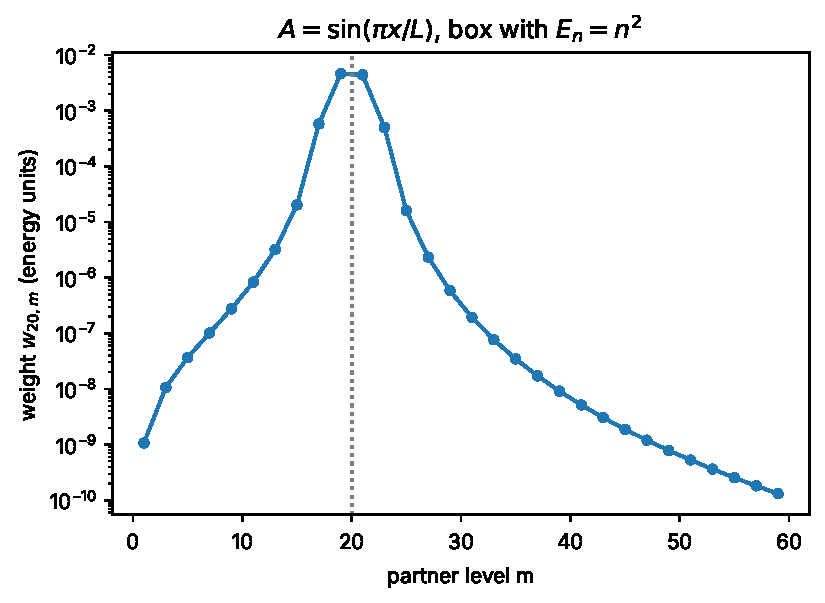
\includegraphics[width=0.85\linewidth]{figs/non-hermitian_locality.pdf}
\caption{Locality of the second-order redistribution. Weights $w_{20,m}=A_{20,m}^2/|E_{20}-E_m|$ for $A=\sin(\pi x/L)$ in the box with $E_n=n^2$ (dimensionless energy units, $\hbar=2m=1$, $L=\pi/2$). Only partners with $20+m$ odd couple. The two neighbors $m=19,21$ carry about 89\% of the total weight summed over partners $m\le400$ (only $m\le60$ are plotted); the weights fall by orders of magnitude within a few levels.}
\label{fig:non-hermitian-locality}
\end{figure}

Locality plus the sum rule give a picture: the imaginary perturbation moves levels toward each other in local groups, and within each neighborhood the pushes approximately cancel. Heuristically, a net shift of a long block of consecutive levels (say 50 of them) is suppressed: most pair contributions cancel inside the block, and only pairs straddling its edges contribute. This is a tendency, not a theorem; the sum rule itself is global, and levels near the edges of a block can exchange shift with partners outside it. This picture motivated a specific hypothesis in the paper, which we discuss in Section~\ref{sec:non-hermitian-paper}.

\begin{checkpoint}
Can the second-order real shifts of an imaginary perturbation raise every one of 652 levels (with the state sum closed over those same 652 levels) by $0.1$?
\end{checkpoint}
\checkanswer{No. The sum rule \eqref{eq:non-hermitian-sumrule} forces the 652 shifts to add to zero, so some must be negative.}

\begin{keyideas}
\item Pair contributions to second-order real shifts are antisymmetric, so they add to zero over any closed set of states, \eqref{eq:non-hermitian-sumrule}.
\item The exact real parts of $D+i\mathsf A$ also add up to $\sum E_n$, by the trace; imaginary perturbations can only redistribute levels.
\item Smooth $A$ couples mainly nearby levels: the redistribution is local, with range set by the highest wavenumber present in $A$.
\end{keyideas}

%======================================================================
\section{The null mode}\label{sec:non-hermitian-null}
%======================================================================

\subsection{A basis function that does nothing}

The absorptive-even basis of the paper is $\phi_k=\cos(k\pi x/L)$, $k=0,1,\dots$, and its first member is $\phi_0=\cos0=1$, a constant. What does a constant imaginary potential $ic_0$ do?

\textbf{Exactly:} by Section~\ref{sec:non-hermitian-decay}, $H_0+ic_0$ has eigenvalues $E_n+ic_0$ and the same eigenfunctions. The real parts do not move at all, at any amplitude.

\textbf{In the tensors:} $(\phi_0)_{nm}=\int\psi_n\psi_m\,\dd x=\delta_{nm}$. In \eqref{eq:non-hermitian-tensor} the sum runs over $m\ne n$, where $(\phi_0)_{nm}=0$. Therefore
\begin{equation}
T^{(n)}_{0l}=T^{(n)}_{l0}=0\qquad\text{for every } n \text{ and } l .
\label{eq:non-hermitian-nullrows}
\end{equation}
The coefficient $c_0$ drops out of $c^\top T^{(n)}c$ entirely: it is a \emph{null mode}, or ``dead parameter'', of the model. Any value of $c_0$ gives the same predictions.

\subsection{When zero is not zero}

On a computer the integral is replaced by a sum over grid points. Recall from Chapter~\ref{ch:eigen} that on a grid of points $x_j$ with spacing $h$ the second-derivative operator becomes a tridiagonal matrix; its eigenvectors give samples $\psi_n(x_j)$, which we scale so that $\sum_j\psi_n(x_j)^2h=1$, the discrete version of normalization (the method is treated in detail later, in Chapter~\ref{ch:finite-differences}). The overlaps are then $(\phi_0)_{nm}=\sum_j\psi_n(x_j)\psi_m(x_j)\,h$, and rounding makes the off-diagonal ones small but not exactly zero. In double precision they come out below $10^{-11}$ in the example of \cref{fig:non-hermitian-nullmode}. If the eigenvectors are stored in single precision (float32, machine epsilon $1.2\times10^{-7}$; Chapter~\ref{ch:asymptotics}), the same overlaps are nonzero at the level of float32 rounding, many orders of magnitude larger.

\begin{figure}[htbp]\centering
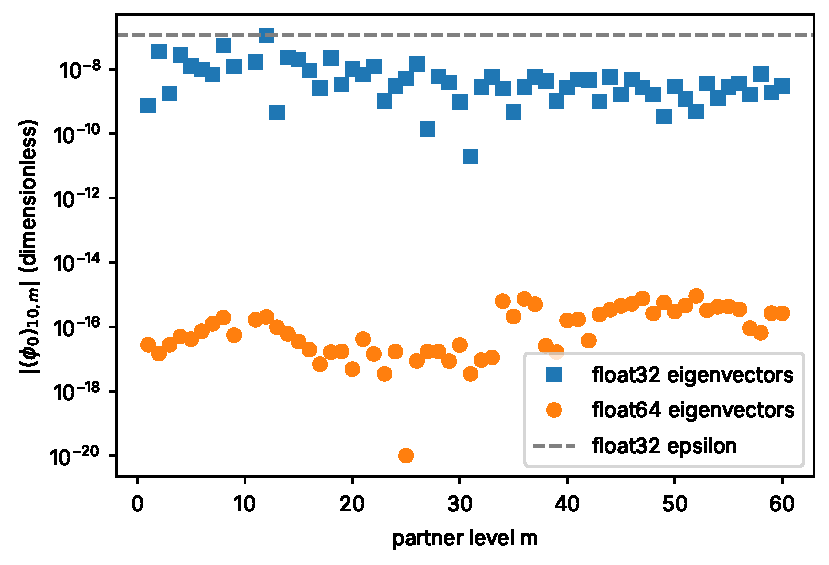
\includegraphics[width=0.85\linewidth]{figs/non-hermitian_nullmode.pdf}
\caption{Overlaps $|(\phi_0)_{10,m}|=|\sum_j\psi_{10}(x_j)\psi_m(x_j)h|$ for $m\ne10$, which are exactly zero analytically, computed from finite-difference box eigenvectors ($L=\pi/2$, $N=400$ grid points, normalization $\sum_j\psi^2h=1$) in double precision (float64) and after rounding the eigenvectors to single precision (float32). The float32 values sit near the float32 rounding scale; the float64 values are many orders of magnitude smaller. Values below $10^{-20}$ are plotted at $10^{-20}$.}
\label{fig:non-hermitian-nullmode}
\end{figure}

\begin{pycode}
import numpy as np
from scipy.linalg import eigh_tridiagonal
L, N = np.pi/2, 400
h = 2*L/(N+1)
d = np.full(N, 2/h**2)            # V = 0 inside the box
e = np.full(N-1, -1/h**2)
E, psi = eigh_tridiagonal(d, e, select="i", select_range=(0, 59))
psi /= np.sqrt(h)                 # now sum(psi**2)*h = 1
O64 = psi.T @ psi * h             # (phi_0)_{nm}: should be the identity
p32 = psi.astype(np.float32)
O32 = (p32.T @ p32) * np.float32(h)
off = ~np.eye(60, dtype=bool)
print("max off-diagonal, float64:", np.abs(O64[off]).max())
print("max off-diagonal, float32:", np.abs(O32[off]).max())
\end{pycode}

Now suppose these noisy overlaps $\eta_{nm}$ are fed into \eqref{eq:non-hermitian-tensor}. The ``zero'' rows become $T^{(n)}_{0l}=\sum_{m\ne n}\eta_{nm}(\phi_l)_{nm}/(E_n-E_m)$, tiny but nonzero, and $T^{(n)}_{00}$ becomes of order $\eta^2$. An optimizer minimizing an in-sample error does not know these entries are noise. If making $c_0$ enormous lowers the error slightly, it will make $c_0$ enormous.

\begin{sample}{How large can a dead parameter grow?}
A toy model: one level, one dead coefficient, $\delta E = -c_0^2\,T_{00}$ with a noise entry $T_{00}=10^{-14}$ (roughly the square of a $10^{-7}$ overlap divided by a spacing of order one). The fit wants $\delta E=y=-0.01$. What value of $c_0$ does an unconstrained least-squares fit choose?

\textbf{Step 1.} Set $-c_0^2T_{00}=y$, so $c_0^2=-y/T_{00}=0.01/10^{-14}=10^{12}$.

\textbf{Step 2.} $c_0=\pm10^6$.
\[
\boxed{|c_0| = 10^6}
\]
A parameter that should be irrelevant becomes the largest number in the model, and the ``improvement'' it buys is entirely an artifact of rounding. In a real fit the cross terms $2c_0\sum_lc_lT^{(n)}_{0l}$, linear in $c_0$, also become order-one numbers when $c_0\sim10^6$ multiplies entries of order $10^{-7}$, so the noise acts as an extra set of fitting functions. This toy is only an order-of-magnitude illustration; it does not reproduce any specific number in the paper.
\end{sample}

\begin{pitfall}
When a model contains a parameter that is exactly null by analysis, set its contribution to exactly zero in code (here: zero the rows and columns \eqref{eq:non-hermitian-nullrows}, or drop $\phi_0$ from the basis). Do not trust the computer to compute zero. A large fitted value for a parameter that should not matter is a warning sign, not a discovery.
\end{pitfall}

\begin{checkpoint}
Why does a constant imaginary potential $ic_0$ leave the real parts of all levels unchanged, even exactly and at large $c_0$?
\end{checkpoint}
\checkanswer{Because $H_0+ic_0$ has the same eigenfunctions as $H_0$, with eigenvalues $E_n+ic_0$: the constant only adds an imaginary number to each eigenvalue.}

\begin{keyideas}
\item A constant imaginary term shifts all eigenvalues by the same imaginary constant; its tensor rows $T^{(n)}_{0l}$ vanish identically.
\item Numerically, analytically-zero entries become rounding noise ($\sim$float32 epsilon in single precision), and an optimizer can drive a dead parameter to huge values to exploit it.
\item Zero null contributions exactly in code.
\end{keyideas}

%======================================================================
\section{PT symmetry}\label{sec:non-hermitian-ptsym}
%======================================================================

\subsection{Parity and time reversal}

We have seen that some non-Hermitian operators, such as $-\dd^2/\dd x^2+x^2+i\epsilon x$, have entirely real spectra. A symmetry explains this. Define two operations on wavefunctions.

\textbf{Parity} $\mathcal P$ reflects space: $(\mathcal P f)(x)=f(-x)$.

\textbf{Time reversal} $\mathcal T$ is complex conjugation: $(\mathcal T f)(x)=f(x)^*$. Why does conjugation reverse time? Suppose $\Psi(x,t)$ solves \eqref{eq:non-hermitian-tdse} with a \emph{real} $V$, and define $\Phi(x,t)=\Psi(x,-t)^*$. Conjugating \eqref{eq:non-hermitian-tdse} gives $-i\,\partial_t\Psi^* = -\Psi^{*\prime\prime}+V\Psi^*$. Evaluate it at time $-t$. By the chain rule, $\partial_t\Phi(x,t) = -(\partial_t\Psi^*)(x,-t)$, so the left side becomes $i\,\partial_t\Phi$, and the equation reads $i\,\partial_t\Phi=-\Phi''+V\Phi$. So $\Phi$ is also a solution: the movie run backwards, conjugated, is a valid motion. If $V$ is complex, the same calculation produces $V^*$ in place of $V$: running a lossy system backwards turns loss into gain.

Combine them: $(\mathcal{PT}f)(x)=f(-x)^*$. Two properties are used below. It is \emph{antilinear}: $\mathcal{PT}(\alpha f)=\alpha^*\,\mathcal{PT}f$ for a complex number $\alpha$. And applying it twice gives back $f$: $(\mathcal{PT})^2f=f$.

\subsection{PT-symmetric Hamiltonians}

$H=-\dd^2/\dd x^2+V(x)$ is \emph{PT-symmetric} if $\mathcal{PT}$ commutes with it: $\mathcal{PT}(Hf)=H(\mathcal{PT}f)$ for all $f$. Let us find the condition on $V$. On one side,
\begin{equation}
\bigl(\mathcal{PT}(Hf)\bigr)(x) = \bigl[-f''(-x)+V(-x)f(-x)\bigr]^* = -f''(-x)^*+V(-x)^*f(-x)^*.
\end{equation}
On the other, let $\chi(x)=f(-x)^*$. Differentiating twice, each derivative brings a factor $-1$ from the chain rule, so $\chi''(x)=f''(-x)^*$, and
\begin{equation}
\bigl(H\chi\bigr)(x) = -f''(-x)^* + V(x)f(-x)^* .
\end{equation}
The two agree for all $f$ if and only if
\begin{equation}
\boxed{\;V(-x)^* = V(x)\;}
\qquad\Longleftrightarrow\qquad V_R \text{ even and } V_I \text{ odd}.
\label{eq:non-hermitian-PTcondition}
\end{equation}
(Write $V=V_R+iV_I$: $V(-x)^*=V_R(-x)-iV_I(-x)$, which equals $V_R(x)+iV_I(x)$ exactly when $V_R(-x)=V_R(x)$ and $V_I(-x)=-V_I(x)$.) Examples: $x^2+i\epsilon x$ is PT-symmetric; so is the famous family $x^2(ix)^{\varepsilon}$ studied by Bender and Boettcher \cite{bender98}.

\subsection{Real eigenvalues when the symmetry is unbroken}

\textbf{Theorem.} Let $H$ be PT-symmetric.
\begin{enumerate}
\item[(a)] If $E$ is an eigenvalue, so is $E^*$. So eigenvalues are real or come in complex-conjugate pairs.
\item[(b)] If an eigenfunction $\psi$ is also an eigenfunction of $\mathcal{PT}$, that is, $\mathcal{PT}\psi=\lambda\psi$ for some number $\lambda$, then $E$ is real.
\end{enumerate}

\textbf{Proof of (a).} Let $H\psi=E\psi$. Then $H(\mathcal{PT}\psi)=\mathcal{PT}(H\psi)=\mathcal{PT}(E\psi)=E^*\,\mathcal{PT}\psi$, using commutation and then antilinearity. And $\mathcal{PT}\psi\ne0$, because applying $\mathcal{PT}$ again gives back $\psi\ne0$. So $\mathcal{PT}\psi$ is an eigenfunction with eigenvalue $E^*$.

\textbf{Proof of (b).} First, $\lambda\ne0$: $\psi=(\mathcal{PT})^2\psi=\mathcal{PT}(\lambda\psi)=\lambda^*\mathcal{PT}\psi=\lambda^*\lambda\psi=|\lambda|^2\psi$, so $|\lambda|=1$. Next compute $\mathcal{PT}(H\psi)$ two ways. Using $H\psi=E\psi$ and antilinearity: $\mathcal{PT}(E\psi)=E^*\lambda\psi$. Using commutation: $H(\mathcal{PT}\psi)=H(\lambda\psi)=\lambda E\psi$. Subtracting, $(E^*-E)\lambda\psi=0$, and since $\lambda\psi\ne0$, $E^*=E$. $\blacksquare$

When every eigenfunction is also a $\mathcal{PT}$ eigenfunction, the symmetry is called \emph{unbroken} and the whole spectrum is real. When some eigenfunctions are not, the symmetry is \emph{broken}, and by (a) those eigenvalues appear in conjugate pairs.

\begin{beyond}
\textbf{Taken on trust:} for the Bender--Boettcher family $-\dd^2/\dd x^2+x^2(ix)^\varepsilon$, the spectrum is entirely real and positive for $\varepsilon\ge0$ (with suitable boundary conditions in the complex plane), and PT symmetry is broken for $\varepsilon<0$. This was found numerically in \cite{bender98}; a rigorous proof was given later, in the mathematical literature that followed that paper, and it is far beyond this book.
\end{beyond}

\subsection{The PT-odd class}

Now take the paper's situation: $V$ is real and even (the Wu--Sprung potential, or the box), and $A$ is real. By \eqref{eq:non-hermitian-PTcondition}, $H_0+iA$ is PT-symmetric exactly when $A$ is \emph{odd}. The paper's ``PT-odd'' class uses the odd basis $\phi_k=\sin((k+1)\pi x/L)$, so every $A=\sum c_k\phi_k$ is odd and every model in the class is PT-symmetric. (The name refers to the imaginary part being odd under parity; the full Hamiltonian is then PT-symmetric.)

For such $A$ the first-order imaginary shift vanishes. In an even potential, each $\psi_n$ is even or odd (Chapter~\ref{ch:bound-states}), so $\psi_n^2$ is even, and $\psi_n^2A$ is odd. The integral of an odd function $g$ over $[-L,L]$ vanishes: $\int_{-L}^{0}g(x)\,\dd x=\int_{0}^{L}g(-y)\,\dd y=-\int_0^Lg(y)\,\dd y$ (substituting $x=-y$), which cancels $\int_0^L g$. Hence $A_{nn}=0$, as we found for the box sines in \eqref{eq:non-hermitian-sinelem}. The same parity argument shows that an odd $A$ couples only states of opposite parity, and an even $A$ only states of the same parity.

So for the PT-odd class the eigenvalue is $E_n-\sum_{m\ne n}|A_{nm}|^2/(E_n-E_m)+\cdots$ with no imaginary part at first or second order; this is what the paper means by ``real spectrum to leading order''. By the theorem, while the symmetry is unbroken the levels stay exactly real. How does it break? Because eigenvalues move continuously with the amplitude and complex eigenvalues must come in conjugate pairs, a simple real eigenvalue cannot leave the real axis on its own. Here is why. Suppose an eigenvalue $E$ is real for amplitudes below some value and complex just above it. By part (a), $E^*$ is then also an eigenvalue just above that value, and as the amplitude decreases back to the departure point both $E$ and $E^*$ approach the same real number. So at the departure point two eigenvalues coincide: a real eigenvalue can leave the axis only by first colliding with another real eigenvalue. This argument uses continuity of the eigenvalues through a coincidence, which the earlier `beyond' box (smoothness for nondegenerate eigenvalues only) does not supply:
\begin{beyond}
\textbf{Taken on trust:} the eigenvalues of a matrix, being the roots of its characteristic polynomial, depend continuously on the matrix entries, even at amplitudes where two of them coincide (though not smoothly there). This is the continuity of polynomial roots in the coefficients; see \cite{trefethen}.
\end{beyond}
Level attraction makes such collisions happen.

\begin{sample}{PT symmetry breaking with two levels}
Return to $M=\begin{pmatrix}E_1&ia\\ia&E_2\end{pmatrix}$ of Section~\ref{sec:non-hermitian-perturb}, now read as an even state 1 and an odd state 2 coupled by an odd $A$. Show that $M$ is PT-symmetric, and describe its spectrum as $a$ grows, for $\Delta=E_2-E_1=1$.

\textbf{Step 1: PT in this basis.} Parity multiplies the even component by $+1$ and the odd one by $-1$: it is the matrix $P=\mathrm{diag}(1,-1)$. Time reversal conjugates components (the basis functions are real). PT symmetry of $M$ means $P\bar MP=M$.

\textbf{Step 2: check.} $\bar M=\begin{pmatrix}E_1&-ia\\-ia&E_2\end{pmatrix}$; multiplying on both sides by $P$ flips the sign of the off-diagonal entries, giving back $\begin{pmatrix}E_1&ia\\ia&E_2\end{pmatrix}=M$.

\textbf{Step 3: spectrum.} From \eqref{eq:non-hermitian-twolevel}, $\lambda_\pm=\bar E\pm\frac12\sqrt{1-4a^2}$.
For $a<\tfrac12$: two real eigenvalues approaching each other (unbroken phase).
At $a=\tfrac12$: they coincide at $\bar E$, and the eigenvectors coincide too (Sample in Section~\ref{sec:non-hermitian-exact}); this is called an \emph{exceptional point}.
For $a>\tfrac12$: a conjugate pair $\bar E\pm\frac i2\sqrt{4a^2-1}$ (broken phase).
\[
\boxed{\text{real for } a<\Delta/2,\quad \text{exceptional point at } a=\Delta/2,\quad \text{conjugate pair for } a>\Delta/2}
\]
Contrast the Hermitian coupling $a$ (without the $i$): $\bar E\pm\frac12\sqrt{1+4a^2}$, always real and always separating. \Cref{fig:non-hermitian-twolevel} plots both parts.
\end{sample}

\begin{figure}[htbp]\centering
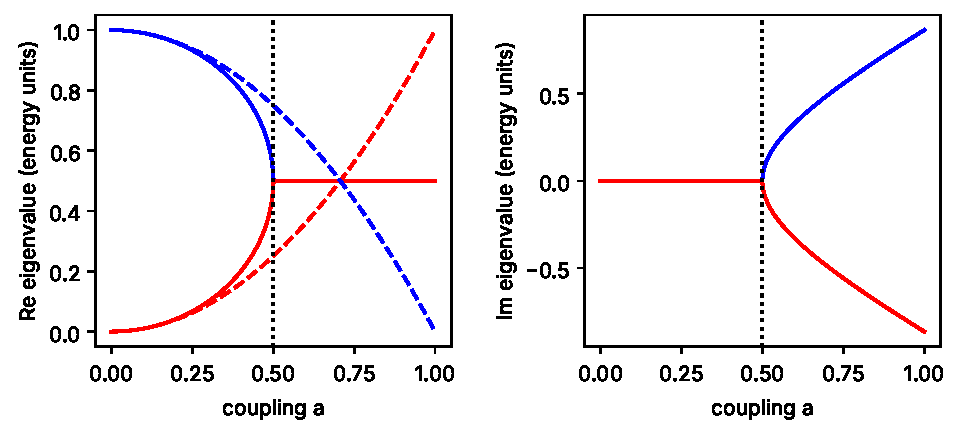
\includegraphics[width=0.85\linewidth]{figs/non-hermitian_twolevel.pdf}
\caption{The two-level model $\begin{pmatrix}0&ia\\ia&1\end{pmatrix}$ (levels $E_1=0$, $E_2=1$, so $\Delta=1$; dimensionless units). (a)~Real parts of the exact eigenvalues (solid) and the second-order predictions $E_1+a^2/\Delta$, $E_2-a^2/\Delta$ (dashed). The levels attract and merge at the exceptional point $a=\Delta/2$ (dotted line); beyond it the exact real parts stay at $1/2$ while the second-order curves keep moving. (b)~Imaginary parts: zero below the exceptional point, a conjugate pair above it.}
\label{fig:non-hermitian-twolevel}
\end{figure}

\subsection{Many levels}

In the box, where the spacing $E_{n+1}-E_n=2n+1$ grows with $n$ while the couplings stay comparable, the lowest levels break first, because they are closest together relative to the coupling. In a spectrum whose spacing shrinks with height (such as the Wu--Sprung levels, Chapter~\ref{ch:wu-sprung}) the opposite ordering is expected for comparable couplings. In the box with $E_n=n^2$ and $A=c\sin(\pi x/L)$, the spacing between levels 1 and 2 is 3, while the coupling is $0.679\,c$ by \eqref{eq:non-hermitian-sinelem}; the two-level estimate puts the break where $0.679\,c\approx1.5$, that is, at $c\approx2.2$. This is only an estimate: in the full truncation each level also couples to other partners, so the true threshold can differ. The numerics below establish only that it lies between $c=1$ and $c=4$; Problem 18 lets you probe $c=2.5$. Higher pairs have larger spacings and slightly smaller couplings. \Cref{fig:non-hermitian-complexplane} shows the exact eigenvalues of a 60-state truncation for several amplitudes, computed as in Section~\ref{sec:non-hermitian-exact}: at $c=1$ all 60 eigenvalues are real to rounding error, and at $c=4$ a complex-conjugate pair has formed near the bottom of the spectrum. The right panel shows the absorptive-even case $A=-g[1+\cos(\pi x/L)]\le0$: every eigenvalue lies on or below the real axis, as Fact 3 of Section~\ref{sec:non-hermitian-matrices} guarantees.

\begin{figure}[htbp]\centering
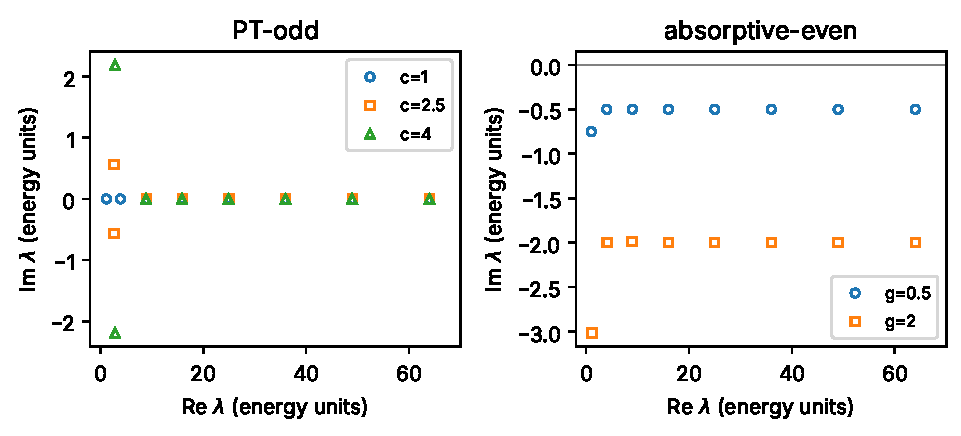
\includegraphics[width=0.85\linewidth]{figs/non-hermitian_complexplane.pdf}
\caption{Exact eigenvalues of $D+i\mathsf A$ in a 60-state truncation of the box with $E_n=n^2$ (dimensionless units, $\hbar=2m=1$, $L=\pi/2$); only the lowest part of the spectrum is shown. Left: PT-odd perturbation $A=c\sin(\pi x/L)$ for $c=1$, $2.5$ and $4$. For $c=1$ all eigenvalues are real; for $c=4$ a complex-conjugate pair has formed near the bottom. Right: absorptive perturbation $A=-g[1+\cos(\pi x/L)]$ for $g=0.5$ and $g=2$; all eigenvalues have $\Im\lambda\le0$.}
\label{fig:non-hermitian-complexplane}
\end{figure}

\begin{checkpoint}
Which of these potentials are PT-symmetric: (a) $x^2+ix$; (b) $x^2+ix^2$; (c) a real even $V(x)$ plus $i\cos(\pi x/L)$?
\end{checkpoint}
\checkanswer{Only (a). In (b) and (c) the imaginary part is even, which violates \eqref{eq:non-hermitian-PTcondition}. Case (c) is the absorptive-even type of the paper.}

\begin{keyideas}
\item $\mathcal{PT}f(x)=f(-x)^*$; $H$ is PT-symmetric iff $V(-x)^*=V(x)$ (real part even, imaginary part odd).
\item Eigenvalues of a PT-symmetric $H$ are real or in conjugate pairs; they are real when the symmetry is unbroken.
\item On an even background, odd $A$ gives a PT-symmetric $H_0+iA$ with $A_{nn}=0$: the paper's PT-odd class.
\item Attraction drives levels together; at an exceptional point they merge and the symmetry breaks into a conjugate pair.
\end{keyideas}

%======================================================================
\section{When second order fails: exact diagonalization and matching}\label{sec:non-hermitian-exact}
% DYK-BEGIN
\begin{didyouknow}{PT Symmetry in the Lab}
Non-Hermitian physics is not just theory. In 2010 Christian R\"uter and collaborators coupled two optical waveguides, one with gain and one with loss, and observed the predicted PT symmetry breaking. As the gain and loss grew past a threshold, the light's behavior changed abruptly. Related ideas now appear in research on lasers and sensors.
\end{didyouknow}
% DYK-END
%======================================================================

\subsection{The radius of the perturbation series}

The two-level model shows precisely how far second order can be trusted. Expand the exact shift \eqref{eq:non-hermitian-twolevelshift} using the Taylor series of $\sqrt{1-x}$ (Chapter~\ref{ch:series}). With $f(x)=(1-x)^{1/2}$: $f(0)=1$, $f'(x)=-\tfrac12(1-x)^{-1/2}$ so $f'(0)=-\tfrac12$, and $f''(x)=-\tfrac14(1-x)^{-3/2}$ so $f''(0)/2=-\tfrac18$. Hence $\sqrt{1-x}=1-\tfrac x2-\tfrac{x^2}{8}-\cdots$ and
\begin{equation}
\lambda_--E_1 = \frac\Delta2\Bigl(\frac x2+\frac{x^2}{8}+\cdots\Bigr) = \frac{a^2}{\Delta}+\frac{a^4}{\Delta^3}+\cdots,
\qquad x=\frac{4a^2}{\Delta^2}.
\label{eq:non-hermitian-series}
\end{equation}
The second-order formula is the first term. The next term, $a^4/\Delta^3$, is smaller by the factor $a^2/\Delta^2=x/4$. So the relative error of second order is about $x/4$ when $x$ is small. The series has radius of convergence 1 in $x$ (Chapter~\ref{ch:series}), so it converges for $|x|<1$, that is, for $a<\Delta/2$, and diverges for $|x|>1$, that is, for $a>\Delta/2$. The radius is set by the exceptional point: at $a=\Delta/2$ the square root vanishes and is not differentiable, and no power series in $a$ can describe the eigenvalue beyond it. This is a general lesson.

\begin{itemize}
\item Second order is accurate when every relevant coupling is small compared with the spacing to the coupled level.
\item As the amplitude grows, second order first becomes inaccurate (here by $x/4$), and then meaningless: past an exceptional point the true real shift stops growing while the formula keeps growing like the square of the amplitude.
\end{itemize}

\subsection{Exact diagonalization}

The remedy is to compute the eigenvalues of $D+i\mathsf A$, or of the finite-difference matrix of $H_0+iA$ (Chapter~\ref{ch:finite-differences}), exactly. The matrix is complex and not Hermitian, so the tridiagonal Hermitian solvers of Chapter~\ref{ch:eigen} do not apply. One uses a general dense eigensolver, \texttt{scipy.linalg.eig}, which handles any square complex matrix. Its cost grows like $\order(K^3)$ for a $K\times K$ matrix, as for dense Hermitian problems, but with a larger constant, and it returns eigenvalues in no particular order.

\begin{pycode}
import numpy as np
from scipy.linalg import eig
K, c = 60, 1.0
n = np.arange(1, K+1)
E = n**2.0                                 # box with L = pi/2
def s1(a, b):                              # (sin_1)_{ab}, Eq. (sinelem)
    if (a+b) % 2 == 0: return 0.0
    return -4/np.pi*(1/(4-(a-b)**2) - 1/(4-(a+b)**2))
A = np.array([[s1(a, b) for b in n] for a in n])
lam, vec = eig(np.diag(E) + 1j*c*A)
match = np.argmax(np.abs(vec)**2, axis=0)  # unperturbed state of each eigvec
order = np.argsort(match)
print(lam[order][:5])
print("one-to-one:", len(set(match)) == K)
\end{pycode}

\subsection{Matching eigenstates by overlap}

The solver returns eigenvalues in an arbitrary order. To compare an exact eigenvalue with the perturbative shift of level $n$, you must know which exact eigenvalue ``belongs'' to level $n$. Sorting by real part fails as soon as two levels cross or merge. The robust method (Chapter~\ref{ch:eigen}) is to \emph{match by overlap}: write each exact eigenvector $v$ in the unperturbed basis (for $D+i\mathsf A$ that is simply its components $v_m$), and assign it to the state $m$ with the largest $|v_m|^2$. For small perturbations, \eqref{eq:non-hermitian-vm} shows that the eigenvector near $E_n$ is $e_n$ plus small admixtures, so the largest component is the $n$-th and the match is unambiguous.

The matching must be \emph{one-to-one}: each unperturbed state receives exactly one exact eigenvector. When two eigenvectors claim the same state (and another state is claimed by none), the perturbed states are no longer identifiable with unperturbed ones. That happens near exceptional points, as the next sample shows, and it is a clear signal that perturbation theory has left its domain.

\begin{sample}{The eigenvector at an exceptional point}
For $M=\begin{pmatrix}E_1&ia\\ia&E_2\end{pmatrix}$ at $a=\Delta/2$, find the eigenvectors and show that overlap matching fails.

\textbf{Step 1.} The double eigenvalue is $\bar E$. Then $M-\bar EI=\begin{pmatrix}-\Delta/2& i\Delta/2\\ i\Delta/2&\Delta/2\end{pmatrix}$, using $E_1-\bar E=-\Delta/2$ and $E_2-\bar E=\Delta/2$.

\textbf{Step 2.} The first row gives $-\tfrac\Delta2v_1+i\tfrac\Delta2v_2=0$, so $v_1=iv_2$. The second row gives $i\tfrac\Delta2v_1+\tfrac\Delta2v_2=i\tfrac\Delta2(iv_2)+\tfrac\Delta2 v_2 = -\tfrac\Delta2v_2+\tfrac\Delta2v_2=0$, consistent. So there is only one independent eigenvector, $v=(i,1)$.

\textbf{Step 3.} $|v_1|^2=|v_2|^2=1$: the single eigenvector overlaps both unperturbed states equally. There is no second eigenvector for the other state.

\textbf{Step 4.} Note also $v^\top v = i^2+1 = 0$ (the transpose, not the conjugate transpose). A nonzero vector whose unconjugated product with itself vanishes is called ``self-orthogonal''; for complex symmetric matrices this happens at exceptional points, as here.
\[
\boxed{v=(i,1),\ \ |v_1|^2=|v_2|^2,\ \ \text{only one eigenvector}}
\]
A $2\times2$ matrix with only one eigenvector cannot be diagonalized, which is why exceptional points are where perturbation theory and overlap matching both break down.
\end{sample}

\subsection{Exact against second order in many levels}

\Cref{fig:non-hermitian-exactvs2nd} repeats the comparison of the two-level sample for the 60-state box. At small amplitude ($c=0.5$) the exact real shifts and the second-order predictions agree closely (their correlation over levels 1--50 exceeds $0.99$, checked in the CHECKS script). At $c=4$, beyond the point where the lowest pair has merged, the second-order predictions no longer describe the operator: they overstate the shifts of the low levels, which in reality cannot move past each other. A fit that optimizes the second-order formula at such amplitudes is optimizing a fiction.

\begin{figure}[htbp]\centering
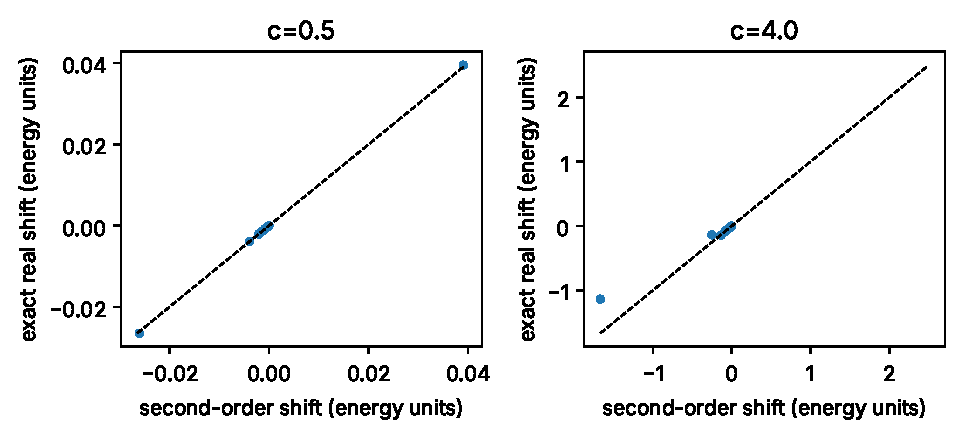
\includegraphics[width=0.85\linewidth]{figs/non-hermitian_exactvs2nd.pdf}
\caption{Exact real shifts $\Re\lambda_n-E_n$ (eigenvectors matched by overlap) against the second-order formula $-c^2T^{(n)}$, for $A=c\sin(\pi x/L)$ in a 60-state box truncation with $E_n=n^2$, levels 1--50 (dimensionless energy units). Left, $c=0.5$: points lie on the diagonal. Right, $c=4$: the lowest levels have merged into a complex pair and the second-order predictions overshoot. Dashed line: exact $=$ second order.}
\label{fig:non-hermitian-exactvs2nd}
\end{figure}

\begin{checkpoint}
In the two-level model with $\Delta=1$, roughly how large is the relative error of the second-order shift at $a=0.1$?
\end{checkpoint}
\checkanswer{About $x/4=a^2/\Delta^2=0.01$, i.e.\ 1\%, matching $0.0100$ versus $0.0101$ in the earlier sample.}

\begin{keyideas}
\item Second order is the first term of a series whose radius is set by the nearest exceptional point; its relative error is about (coupling/spacing)$^2$.
\item Beyond an exceptional point the exact real shift saturates while the second-order formula keeps growing.
\item Non-Hermitian matrices need a general eigensolver (\texttt{scipy.linalg.eig}); eigenvalues come unordered and are matched to unperturbed states by largest overlap, which must be one-to-one.
\item Failure of one-to-one matching signals that perturbation theory has broken down.
\end{keyideas}

%======================================================================
\section{Paper connection}\label{sec:non-hermitian-paper}

\paragraph{Vocabulary.} Secs.~V and V A of the paper use a few terms from later chapters. Each model is fitted to the zeros $1,\dots,400$. The misfit is measured as an \emph{in-sample rms}: the root mean square, over the fitted zeros, of the difference between model level and target, each difference divided by the local mean spacing $\mathrm{gap}_n$ (the average distance between neighboring zeros near zero $n$; Chapter~\ref{ch:counting-zeros}), so errors are quoted ``in mean spacings''. The \emph{target fluctuation} $\mathrm{fluc}_n$ is the amount by which level $n$ must move away from its unperturbed value $E_n$ to land on its target. The \emph{null} is the misfit with no perturbation at all ($c=0$). The \emph{floor} is the lowest in-sample rms the optimizer reaches. The \emph{surrogate} is the second-order formula $-c^\top T^{(n)}c$, used during fitting in place of the exact spectrum.
%======================================================================

\paragraph{The two model classes (Sec.~II E).} The paper perturbs the Wu--Sprung Hamiltonian $H$ (Chapter~\ref{ch:wu-sprung}) as $H\to H+iA$ with $A=\sum_kc_k\phi_k$ a real multiplication operator, exactly our \eqref{eq:non-hermitian-HiA} and \eqref{eq:non-hermitian-Aexpand}. The \emph{PT-odd} class uses $\phi_k=\sin((k+1)\pi x/L)$; every such $A$ is odd (a sum of sines); since the Wu--Sprung potential is even, Section~\ref{sec:non-hermitian-ptsym} shows that $H+iA$ is then PT-symmetric and $A_{nn}=0$, which is the paper's ``real spectrum to leading order''. The \emph{absorptive-even} class uses $\phi_k=\cos(k\pi x/L)$, ``modelling $-i\Gamma/2$'': by \eqref{eq:non-hermitian-first} it produces first-order widths $\Gamma_n=-2A_{nn}$, which are nonnegative for every state if $A\le0$ pointwise (Fact 3 of Section~\ref{sec:non-hermitian-matrices}). That is the paper's ``physical constraint $\Gamma\ge0$ (i.e.\ $A\le0$ pointwise)''.

\paragraph{Eq.~(5).} The paper's Eq.~(5), $\delta E_n=-\sum_{m\ne n}|A_{nm}|^2/(E_n-E_m)=-c^\top T^{(n)}c$, is our \eqref{eq:non-hermitian-second} and \eqref{eq:non-hermitian-tensor}; the minus sign is the $i^2$ of Section~\ref{sec:non-hermitian-perturb}. The state sum runs ``over all 652 basis states with $E\le1000$'', and the paper notes that ``truncating at 500 states measurably biases the top levels''. Section~\ref{sec:non-hermitian-perturb} explains the direction: partners above a level push it up (attraction), so cutting them off removes upward pushes from the levels near the cutoff and biases them downward (the topmost level keeps only downward pushes). App.~A step 9 records the tensor computation, with eigenvectors normalized as $\sum\psi^2dx=1$. The fit (App.~A step 10) minimizes residuals $(\mathrm{fluc}_n+c^\top T^{(n)}c)/\mathrm{gap}_n$ using the Jacobian $2(T^{(n)}c)_k/\mathrm{gap}_n$, the gradient derived in Section~\ref{sec:non-hermitian-tensor}, with six random restarts because the problem is nonconvex.

\paragraph{Safeguard (i) and the null mode (Sec.~II E, Sec.~V).} The paper says the even basis ``contains the exactly-null constant mode $\phi_0=1$ (a constant $iA$ shifts all eigenvalues by the same imaginary constant and has zero second-order real shift); its analytically-vanishing tensor rows are zeroed exactly rather than left as float32 noise''. This is Section~\ref{sec:non-hermitian-null}. Sec.~V reports what happened before the repair: the absorptive-even floor sat at $0.2322$, ``spuriously close to the PT-odd value'' $0.2321$, because ``the optimizer had driven the exactly-null constant mode to $c_0\approx2.2\times10^{6}$, harvesting in-sample improvement from float32 noise''. With the artifact removed, the absorptive-even floor is $0.2358$; the null is $0.2438$ (all in-sample rms on zeros 1--400, in mean spacings). Our toy sample produced $|c_0|\sim10^6$ by the same mechanism; Problem 16 estimates why such a value turns noise into order-one shifts.

\paragraph{Safeguard (iii), exact diagonalization (Sec.~V, Fig.~5).} Under ``The optimizer left the perturbative regime'', Sec.~V reports that at the fitted amplitude ``corr(exact, second-order) drops to $+0.14$/$+0.18$ (odd/even), the surrogate overstates shift magnitudes twofold (Fig.~5, left), and 3\% of eigenstates can no longer be matched one-to-one to unperturbed states''. Each phrase now has a meaning for you: the exact spectrum comes from dense complex \texttt{eig} on a grid of $N=2500$ points (App.~A step 11), states are matched by overlap as in Section~\ref{sec:non-hermitian-exact}, and loss of one-to-one matching signals strong mixing of unperturbed states, of which exceptional points (Section~\ref{sec:non-hermitian-ptsym}) are the extreme case; the paper does not identify which occurs. The factor of two recalls our two-level sample, where at $a=\Delta$ second order gave $1.0$ against an exact $0.5$ (a toy illustration, not an explanation of the paper's specific factor). Scoring the exact spectra in-sample gives $0.2523$ and $0.2477$, ``worse than the null $0.2438$''; ``the $0.232$ floor was a property of the surrogate, not of any operator''. At quarter amplitude the surrogate is accurate (corr $+0.88$/$+0.94$); at quarter amplitude every coupling $A_{nm}$ is 4 times smaller, so the coupling-to-spacing ratio falls fourfold, the second-order shifts fall 16-fold (they scale as $c^2$, Section~\ref{sec:non-hermitian-tensor}), and the relative error of second order, of order (coupling/spacing)$^2$ by Section~\ref{sec:non-hermitian-exact}, falls about 16-fold. Sec.~V also states that ``58\% of its widths have the wrong sign'' for the unconstrained absorptive-even fit, which by Fact 3 means the fitted $A$ was positive (gain) somewhere, and by $\Gamma_n=-2A_{nn}$ that its average weighted by $|\psi_n|^2$ was positive for more than half the states.

\paragraph{Safeguard (ii), amplitude balls.} The fair refits restrict $\lVert c\rVert\le R$ (App.~A step 10: projection after each step, restarts with spread $R/20$, sign penalty $10^4\int\max(A,0)^2\,dx$) so that second order stays valid. Their floors are within $0.4$--$4.8\%$ of the null (Fig.~5, right); the $R=4$ solutions pass exact verification (corr $+0.93$/$+0.995$, all states matched), with exact-spectrum in-sample gains of $1.9\%$ (odd) and $0.6\%$ (even). The paper concludes that these families, ``treated fairly, are empirically inert on this problem''.

\paragraph{Sum rule and locality (Sec.~V, V A).} The paper verifies $\sum_n\delta E_n=0$ to $3.6\times10^{-15}$ (odd) and $1.4\times10^{-14}$ (even) at the fitted coefficients (Sec.~V A), our theorem \eqref{eq:non-hermitian-sumrule}, and reports locality with exactly our weights \eqref{eq:non-hermitian-weights}: half the weight within $|n-m|\le5$ (odd) and $\le10$ (even), 90\% within about 60 levels. The ``block-coherence'' hypothesis was that, since the redistribution is local and sums to zero, the model can only produce locally mean-free patterns and the floor equals the rms of the locally averaged part of the target. Sec.~V A refutes it: the block-coherent rms is $0.108,0.049,0.033,0.035,0.019$ for windows $w=3,5,7,9,13$, ``far below the observed floors''. The paper's own summary is that ``the floor is simply the null minus a small capture''.

\paragraph{Status.} The paper calls Sec.~V ``a methodological stress test of a second model class''; its Hermitian conclusions do not depend on it, and Sec.~VI states that this analysis ``was not rerun for this revision''. Its general lesson is the one this chapter's mathematics makes concrete: ``A surrogate improvement is not an operator-level result until the exact spectrum of the fitted operator confirms it.''

%======================================================================
\section{Summary}
%======================================================================
\begin{itemize}
\item The imaginary part of a potential changes total probability at rate $2\int V_I|\Psi|^2\,\dd x$, \eqref{eq:non-hermitian-dPdt}; a constant $-\Gamma/2$ gives decay $e^{-\Gamma t}$, \eqref{eq:non-hermitian-expdecay}.
\item $\Im E$ is the state-weighted average of $V_I$, \eqref{eq:non-hermitian-ImE}; $V_I\le0$ implies all widths $\Gamma=-2\Im E\ge0$.
\item In the real eigenbasis, $H_0+iA$ is the complex symmetric matrix $D+i\mathsf A$, \eqref{eq:non-hermitian-M}; its eigenvalues' real parts sum to $\sum E_n$, \eqref{eq:non-hermitian-tracerule}, and are even in the amplitude, \eqref{eq:non-hermitian-parity-in-c}.
\item General second order: $\sum_{m\ne n}W_{nm}W_{mn}/(E_n-E_m)$, \eqref{eq:non-hermitian-generalPT}. For $W=iA$: first order $iA_{nn}$, \eqref{eq:non-hermitian-first}; leading real shift $-\sum|A_{nm}|^2/(E_n-E_m)$, \eqref{eq:non-hermitian-second}: level attraction.
\item Quadratic form $\delta E_n=-c^\top T^{(n)}c$, \eqref{eq:non-hermitian-tensor}; box matrix elements \eqref{eq:non-hermitian-coselem}, \eqref{eq:non-hermitian-sinelem}.
\item Sum rule $\sum\delta E_n=0$ over a closed set, \eqref{eq:non-hermitian-sumrule}; locality of weights \eqref{eq:non-hermitian-weights}.
\item The constant mode is null: $T^{(n)}_{0l}=0$, \eqref{eq:non-hermitian-nullrows}; zero it in code.
\item PT symmetry iff $V(-x)^*=V(x)$, \eqref{eq:non-hermitian-PTcondition}; spectra real or in conjugate pairs; breaking at exceptional points.
\item Second order is a series with radius set by the nearest exceptional point, \eqref{eq:non-hermitian-series}; verify with exact diagonalization and one-to-one overlap matching.
\end{itemize}

%======================================================================
\section{Problems}
%======================================================================
\begin{problemlist}
\prob{1}{A uniform absorber with $\Gamma=0.1$ acts on a particle in a box. Find the half-life and the fraction remaining at $t=20$.}
\prob{1}{An eigenvalue is $E=5-0.3i$. What are the level, the width, and the mean lifetime?}
\prob{1}{Find the eigenvalues of $\begin{pmatrix}0&i\\i&0\end{pmatrix}$ and of $\begin{pmatrix}0&1\\1&0\end{pmatrix}$. Comment.}
\prob{1}{Using \eqref{eq:non-hermitian-PTcondition}, decide which are PT-symmetric: (a) $ix^3$; (b) $x^4+ix^3$; (c) $x^2+i\sin x$; (d) $x^2-i$.}
\prob{1}{Explain in one sentence why, at second order, an imaginary perturbation lowers the highest state of a truncated basis.}
\prob{2}{In the RE3 box, the absorber is $A=-g[1-\cos(\pi x/L)]$ (zero at the center, strongest at the walls). Find the first-order widths of all levels. Which level is longest-lived, and why physically?}
\prob{2}{Starting from \eqref{eq:non-hermitian-dPdt}, derive \eqref{eq:non-hermitian-expdecay} and show that the decay rate does not depend on the state.}
\prob{2}{Show that at the exceptional point the $2\times2$ matrix of Section~\ref{sec:non-hermitian-exact} satisfies $(M-\bar EI)^2=0$ but $M-\bar EI\ne0$.}
\prob{2}{In the two-level model with $\Delta=1$ and $a=0.3$, compute the exact shift of the lower level and the second-order prediction.}
\prob{2}{Continue Problem 9: add the fourth-order term $a^4/\Delta^3$ of \eqref{eq:non-hermitian-series}. How close is the sum to the exact shift?}
\prob{2}{For the four-state sample of Section~\ref{sec:non-hermitian-tensor}, show algebraically (without numbers) that $T^{(1)}+T^{(2)}+T^{(3)}+T^{(4)}=0$.}
\prob{2}{Prove that in an even potential an odd $A$ has $A_{nm}=0$ whenever $\psi_n$ and $\psi_m$ have the same parity.}
\prob{2}{Verify numerically the gradient formula $\partial(c^\top Tc)/\partial c_k=2(Tc)_k$ for $T=\begin{pmatrix}1&2\\2&-3\end{pmatrix}$ and $c=(0.5,1)$ by finite differences.}
\prob{2}{Find the eigenvalues of $\begin{pmatrix}1&i\\i&2\end{pmatrix}$ and check the trace rule \eqref{eq:non-hermitian-tracerule}.}
\prob{2}{(Paper) Sec.~II E says that truncating the state sum of Eq.~(5) at 500 states instead of 652 ``measurably biases the top levels''. Predict the sign of the bias on levels near 400--500.}
\prob{2}{(Paper) With $c_0\approx2.2\times10^6$ (Sec.~V) and noisy null-row entries of order $10^{-7}$, estimate the size of a cross term $2c_0T^{(n)}_{0l}c_l$ for $c_l\sim1$, and compare with a mean spacing (of order one at these heights).}
\prob{3}{Add state 5 ($E_5=25$) to the four-state sample. Compute the new $T^{(4)}$ and $\delta E_4$, and check that the five shifts still sum to zero.}
\prob{2}{Using numpy, rebuild \cref{fig:non-hermitian-complexplane} and find, for $c=2.5$, how many eigenvalues of the 60-state truncation have $|\Im\lambda|>10^{-6}$.}
\prob{2}{Using numpy, form the 60-state tensors $T^{(n)}$ for the two-function basis $\sin(\pi x/L)$, $\sin(2\pi x/L)$ in the box with $E_n=n^2$, using \eqref{eq:non-hermitian-sinelem} with $j=1,2$. Draw a random $c=(c_0,c_1)$ and verify that $\sum_n c^\top T^{(n)}c=0$ to rounding.}
\prob{2}{Using qmnt or numpy, repeat the null-mode experiment of \cref{fig:non-hermitian-nullmode} with $N=2000$. Does the float32 noise grow or shrink?}
\prob{3}{In the two-level model, show that for $a\ge\Delta/2$ the ratio of the second-order real shift to the exact real shift is $2a^2/\Delta^2$.}
\prob{2}{(Paper) Sec.~V reports that 58\% of the unconstrained absorptive-even widths had the wrong sign. Using Fact 3 of Section~\ref{sec:non-hermitian-matrices}, what does this say about the fitted $A(x)$?}
\prob{2}{(Paper) Sec.~V checks the surrogate at quarter amplitude. By what factor are all second-order shifts reduced?}
\prob{2}{(Paper) The fair $R=4$ odd fit gained $1.9\%$ over the null $0.2438$ in exact-spectrum in-sample rms. What rms does this imply, and compare with the exact-verified anchor of App.~A.}
\prob{3}{Show that for any $A$, the sum of first-order widths over a closed set of $K$ states is $-2\sum_nA_{nn}$, and that for $A=-g$ constant it equals $2gK$.}
\prob{2}{Write down a $3\times3$ PT-symmetric matrix (even, odd, even states) with an odd coupling and verify $P\bar MP=M$.}
\prob{3}{Prove the trace rule for $3\times3$ matrices by expanding $\det(\lambda I-M)$ and comparing the $\lambda^2$ coefficient with $\prod(\lambda-\lambda_i)$.}
\prob{3}{Use $\langle n|x|n+1\rangle=\sqrt{(n+1)/2}$ and $E_n=2n+1$ to show from \eqref{eq:non-hermitian-second} that every oscillator level shifts by $+\epsilon^2/4$ under $i\epsilon x$.}
\prob{2}{(Paper) Sec.~V A verifies the sum rule to $3.6\times10^{-15}$ with 652 states. Assuming the individual shifts are of order one in the paper's units, compare with $652$ times double-precision machine epsilon. Is the verification consistent with rounding?}
\prob{3}{(Paper, open-ended) Explain in your own words why locality plus the sum rule suggested the block-coherence hypothesis, and why the numbers in Sec.~V A refute it.}
\prob{1}{What width $\Gamma$ makes the probability fall by a factor $e$ in time 100?}
\end{problemlist}

%======================================================================
\section{Answers to selected problems}
%======================================================================
\begin{description}
\item[1.] $t_{1/2}=\log2/0.1=6.931$; remaining $e^{-2}=0.1353$.
\item[2.] Level $5$, width $\Gamma=-2\Im E=0.6$, lifetime $1/0.6=1.667$.
\item[3.] Discriminant $4(i)(i)=-4$, so $\lambda=\pm i$; the real version gives $\pm1$. The factor $i$ on the couplings turns repulsion into a complex pair.
\item[4.] (a) yes (odd imaginary part, zero real part); (b) yes; (c) yes ($\sin$ is odd); (d) no (constant imaginary part is even).
\item[5.] All its partners lie below it, so each term $-|A_{Km}|^2/(E_K-E_m)$ is negative.
\item[7.] With $V_I=-\Gamma/2$, $\dd P/\dd t=-\Gamma\int|\Psi|^2=-\Gamma P$; the solution is $P(0)e^{-\Gamma t}$ for any initial state.
\item[9.] $x=0.36$; exact $\tfrac12(1-0.8)=0.1$; second order $0.09$.
\item[11.] Each pair $(n,m)$ enters $T^{(n)}$ with $1/(E_n-E_m)$ and $T^{(m)}$ with $1/(E_m-E_n)$, same numerator; they cancel.
\item[13.] $Tc=(2.5,-2)$, so gradient $(5,-4)$; central differences reproduce it to rounding.
\item[15.] Missing partners above would push the top levels up; without them the top levels are biased downward.
\item[17.] $(\sin_1)_{45}=-0.4410$, $(\sin_1)_{25}=0.2264$; $T^{(4)}=0.0318-0.4410^2/9=0.0102$, so $\delta E_4=-0.0102\,c^2$. The five shifts still sum to zero.
\item[19.] The total is zero to rounding error: its magnitude is below $10^{-12}$ times the largest $|\delta E_n|$.
\item[21.] Exact real shift $\Delta/2$; second order $a^2/\Delta$; ratio $2a^2/\Delta^2$ ($=2$ at $a=\Delta$).
\item[23.] Shifts scale as $c^2$: factor $1/16=0.0625$.
\item[25.] $\Gamma_n=-2A_{nn}$; summing gives $-2\sum A_{nn}=-2\,\mathrm{tr}\,\mathsf A$; for $A=-g$, $A_{nn}=-g$ and the sum is $2gK$.
\item[27.] Both expressions give $\lambda^3-(\sum\lambda_i)\lambda^2+\dots$ and $\lambda^3-(M_{11}+M_{22}+M_{33})\lambda^2+\dots$; equate coefficients.
\item[29.] Assuming shifts of order one, the rounding scale is about $652\times2.2\times10^{-16}=1.4\times10^{-13}$; the verified $3.6\times10^{-15}$ is below that scale, consistent with pure rounding (under that assumption, since the paper does not report the size of the individual shifts).
\item[31.] $\Gamma=1/100=0.01$.
\end{description}
